% !TeX program = lualatex
\documentclass[12pt,a4paper]{article}

% ========= حزمة =========
\usepackage[english, bidi=default, layout=counters]{babel}
\usepackage{amsmath,amssymb,amsfonts,mathtools}
\usepackage{amsthm}
\usepackage{geometry}
\geometry{left=1.0cm,right=1.0cm,top=1.25cm,bottom=3.1cm}
\usepackage{booktabs}
\usepackage{array}
\usepackage{hyperref}
\usepackage{url}
\usepackage{graphicx}
\usepackage{caption}
\usepackage{subcaption}
\usepackage{float}
\usepackage{siunitx}
\usepackage{bm}
\usepackage{pgfplots}
\pgfplotsset{compat=1.18}
\usepackage{xcolor}
\usepackage{titlesec}
\usepackage{fancyhdr}
\usepackage{microtype}
\usepackage{fontspec}
\usepackage{parskip}
\usepackage{physics}
\usepackage{tikz}
\usetikzlibrary{arrows.meta, positioning, calc, shapes.geometric, decorations.pathmorphing, patterns, quotes, angles, 3d}
\usepackage{makecell}
\usepackage{ragged2e}
\usepackage{tabularx}
\usepackage{longtable}

% ========= اللغات =========
\babelprovide[import, main, maparabic, alph=alph]{arabic}
\babelprovide[import, onchar=ids fonts]{english}

% ========= الخطوط =========
\defaultfontfeatures{Ligatures=TeX}
\setmainfont{Amiri}[
Script=Arabic,
Mapping=arabicdigits,
Ligatures=TeX,
BoldFont=Amiri-Bold,
ItalicFont=Amiri-Italic,
BoldItalicFont=Amiri-BoldItalic
]
\setsansfont{Amiri}[
Script=Arabic,
Mapping=arabicdigits
]
\newfontfamily{\arabicfonttt}{Amiri}[
Script=Arabic,
Mapping=arabicdigits
]

% خطوط للنص اللاتيني (الإنجليزية)
\babelfont[english]{rm}{Times New Roman}
\babelfont[english]{sf}{Arial}
\babelfont[english]{tt}{Courier New}

% ========= ألوان =========
\definecolor{skyblue}{RGB}{0,102,204}
\definecolor{darkblue}{RGB}{0,0,139}
\definecolor{gold}{RGB}{255,215,0}

% ========= أوامر YUCT =========
\newcommand{\eps}{\varepsilon}
\newcommand{\kappac}{\kappa_c}
\newcommand{\Keff}{K_{\mathrm{eff}}}
\newcommand{\betaf}{\beta}
\newcommand{\df}{d_{\!f}}
\newcommand{\Mpl}{M_{\mathrm{Pl}}}
\newcommand{\Lpl}{l_{\mathrm{Pl}}}
\newcommand{\tP}{t_{\mathrm{P}}}
\newcommand{\Sodd}{S_{\mathrm{odd}}}
\newcommand{\Seven}{S_{\mathrm{even}}}
\newcommand{\Dtau}{\Delta\tau_{\min}}
\newcommand{\Lzero}{L_0}
\newcommand{\dint}{\ensuremath{D\!+\!I\!\cdot\!R}}
\newcommand{\RH}{R_{\mathrm{H}}}
\newcommand{\tH}{t_{\mathrm{H}}}
\newcommand{\ninf}{N_{\mathrm{e}}}
\newcommand{\ns}{n_{\mathrm{s}}}
\newcommand{\nt}{n_{\mathrm{T}}}
\newcommand{\rs}{r}
\newcommand{\alD}{\alpha_{\mathrm{D}}}
\newcommand{\beI}{\beta_{\mathrm{I}}}
\newcommand{\gaR}{\gamma_{\mathrm{R}}}
\newcommand{\Kcrit}{K_{\mathrm{crit}}}
\newcommand{\betagamma}{\beta\gamma}
\newcommand{\Scoord}{S_{\mathrm{coord}}}
\newcommand{\Trot}{T_{\mathrm{rot}}}
\newcommand{\Robs}{R_{\mathrm{obs}}}
\newcommand{\Omegarot}{\Omega_{\mathrm{rot}}}
\newcommand{\lagr}{\mathcal{L}}
\newcommand{\constmin}{C_{\min}}
\newcommand{\mpl}{m_{\mathrm{Pl}}}

% ========= بيئات النظرية =========
\newtheorem{theorem}{نظرية}[section]
\newtheorem{lemma}{ليما}[section]
\newtheorem{corollary}{نتيجة}[section]
\newtheorem{definition}{تعريف}[section]
\newtheorem{axiom}{مسلمة}[section]
\newtheorem{proposition}{اقتراح}[section]
\newtheorem{remark}{ملاحظة}[section]
\newtheorem{prediction}{تنبؤ}[section]

% ========= تنسيق العناوين =========
\titleformat{\section}{\LARGE\bfseries\color{darkblue}}{\thesection}{1em}{}
\titleformat{\subsection}{\Large\bfseries\color{darkblue}}{\thesubsection}{1em}{}
\titleformat{\subsubsection}{\normalsize\itshape}{\thesubsubsection}{1em}{}

% ========= رؤوس وتذييلات =========
\fancypagestyle{firstpage}{%
	\fancyhf{}%
	\renewcommand{\headrulewidth}{0pt}%
	\renewcommand{\footrulewidth}{0pt}%
	\fancyfoot[C]{%
		\begin{minipage}[t]{\textwidth}
			\centering
			\textcolor{gold}{\rule{\textwidth}{1.6pt}}\\[5pt]
			{\small \textsuperscript{1}أبحاث ياكوشيف، \url{https://yuct.org/}} \hfill
			{\small بروتوكول YPSDC: \url{https://ypsdc.com/}}\\[-2pt]
			\textcolor{gold}{\rule{\textwidth}{1.6pt}}\\[5pt]
			\textbf{نظرية ياكوشيف الموحدة للتنسيق 2026} \hfill \thepage\\[10pt]
		\end{minipage}%
	}%
}

\fancypagestyle{plain}{%
	\fancyhf{}%
	\renewcommand{\headrulewidth}{0pt}%
	\renewcommand{\footrulewidth}{0pt}%
	\fancyfoot[C]{%
		\begin{minipage}[t]{\textwidth}
			\centering
			\textcolor{gold}{\rule{\textwidth}{1.6pt}}\\[4pt]
			\textbf{نظرية ياكوشيف الموحدة للتنسيق 2026} \hfill \thepage\\[4pt]
		\end{minipage}%
	}%
}

\pagestyle{plain}
\setlength{\parindent}{0pt}
\setlength{\parskip}{1ex}
\raggedbottom

\hypersetup{
	colorlinks=true,
	linkcolor=blue,
	citecolor=blue,
	urlcolor=blue,
}

% ========= رأس المقال (شعار YUCT) =========
\newcommand{\makeheader}{%
	\noindent
	\begin{minipage}{0.17\textwidth}
		\raggedright
		{\sffamily\bfseries\color{skyblue}\fontsize{46}{46}\selectfont YUCT}%
	\end{minipage}%
	\hspace{30pt}
	\begin{minipage}{0.32\textwidth}
		\raggedright
		{\sffamily\fontsize{11}{13}\selectfont نظرية ياكوشيف\\ الموحدة\\ للتنسيق}%
	\end{minipage}%
	\hfill
	\begin{minipage}{0.38\textwidth}
		\raggedleft
		{\sffamily\bfseries ملحق \(\Omega\). الإصدار 2.1}\\
		{\sffamily نُشر في أبريل 2026}\\
		{\sffamily\footnotesize \url{https://doi.org/10.5281/zenodo.18444598}}%
	\end{minipage}
	\par\vspace{5pt}
	\noindent\textcolor{gold}{\rule{\textwidth}{1.6pt}}
	\par\vspace{0pt}
}

\begin{document}
	\thispagestyle{firstpage}
	\makeheader
	
	\vspace{0cm}
	{\LARGE\bfseries ملحق \(\Omega\): الكتلة الحرجة للانفجار العظيم المحلي كانقال طور تنسيقي، والدوران الشامل للكون، وعمره الأدنى الجديد من نصف قطر دوران ثنائي القطب \par}
	\vspace{0.2cm}
	
	{\large أليكسي ف. ياكوشيف\footnote{أبحاث ياكوشيف، \url{https://yuct.org/}}} \\
	\vspace{0.0cm}
	
	{\color{darkblue}\textbf{\LARGE المستخلص}} \par
	{\large
		\noindent
		تفترض نظرية ياكوشيف الموحدة للتنسيق (YUCT) أن كوننا المرصود نشأ كانقال طور محلي – "انفجار عظيم" – داخل كون أكبر يدور أبدياً. لا يستطيع علم الكون القياسي التنبؤ بالكتلة أو مقياس الطاقة الابتدائيين للانفجار العظيم، ويعامله كشرط حدي متفرد. في وثيقة أوميغا هذه نوحد ثلاث ركائز أساسية لـ YUCT: (1) اشتقاق الكتلة الحرجة \(M_{\mathrm{crit}}\) التي تُطلق الانفجار العظيم المحلي من المسلمات الأساسية؛ (2) الطور التضخمي كانقال طور تنسيقي، بما في ذلك البصمات الرصدية الفريدة؛ و(3) الدوران الشامل للكون كأصل لثنائي قطب CMB وحد أدنى جديد للعمر الكوني. انطلاقاً من تعريف YPSDC لكفاءة التنسيق والطبيعة الكسيرية لشبكة التنسيق، نُثبت قانون القياس \(K_{\mathrm{eff}} \propto R^{\beta d_f/2}\) مع \(\beta = 2/3\) والبعد الكسيري \(d_f = 2.2\). وبتطبيق هذا على منطقة مرتبطة جذبوياً قبل الانهيار نجد \(M_{\mathrm{crit}} = 3 M_{\mathrm{Pl}} \approx 6.5 \times 10^{-8}\;\text{kg}\). المسلمات نفسها تحكم ديناميك التضخم، متنبئةً بـ \(n_s \approx 0.965\)، \(r \approx 0.07\)، ولا غاوسية مميزة \(f_{\mathrm{NL}}^{\mathrm{local}} \approx 1.12\). الدوران الشامل للكون، المستنتج من نمو ثنائي قطب CMB مع الانزياح نحو الأحمر، يؤدي إلى دور دوران \(T_{\mathrm{rot}} \approx 2.3 \times 10^{14}\) سنة، متجاوزاً بكثير العمر الكوني القياسي. إن اتساق هذه الخطوط الثلاثة المستقلة من الأدلة – الكتلة الحرجة المجهرية، تضخم الكون المبكر، والدوران الحالي – يُشكل برهان تلاقٍ لـ YUCT. نقدم اشتقاقات مفصلة، وتنبؤات قابلة للتكذيب، ومعايير تفنيد صريحة لكل مكون. تؤسس وثيقة أوميغا هذه YUCT كإطار تنبؤي موحد يربط الجاذبية الكمومية، وعلم الكون، والبنية واسعة النطاق للكون.
	}
	
	\vspace{0.1cm}
	\noindent
	{\color{darkblue}\textbf{الكلمات المفتاحية:}} YUCT، الكتلة الحرجة، الانفجار العظيم، انتقال طور تنسيقي، التضخم، اللاغاوسية، الدوران الشامل، ثنائي قطب CMB، البعد الكسيري، الحلقة الجبرية، قابلية التكذيب.
	
	\vspace{0.1cm}
	\noindent
	{\color{darkblue}\textbf{الاقتباس:}} ياكوشيف أ.ف. أوميغا: الكتلة الحرجة للانفجار العظيم المحلي كانقال طور تنسيقي والدوران الشامل للكون. 2026. DOI: \url{https://doi.org/10.5281/zenodo.18444598} (هذا المجلد).
	
	\vspace{0.4cm}
	\clearpage
	\tableofcontents
	\clearpage
	
	%%%%%%%%%%%%%%%%%%%%%%%%%%%%%%%%%%%%%%%%%%%%%%%%%%%%%%%%%%%%%%%%%%%%%%%%%%%
	% الجزء الأول: الكتلة الحرجة للانفجار العظيم المحلي
	%%%%%%%%%%%%%%%%%%%%%%%%%%%%%%%%%%%%%%%%%%%%%%%%%%%%%%%%%%%%%%%%%%%%%%%%%%%
	\part{الكتلة الحرجة للانفجار العظيم المحلي}
	\label{part:I}
	
	\section{مقدمة}
	
	يبقى أصل الكون أعمق لغز في علم الكون. في إطار النسبية العامة القياسية، الانفجار العظيم هو حدث متفرد ذو كثافة وحرارة لانهائيتين، ولا يقدم أي قدرة تنبؤية فيما يتعلق بالكتلة أو مقياس الطاقة الابتدائيين. مقاربات الجاذبية الكمومية (نظرية الأوتار، الجاذبية الكمومية الحلقية) تستبدل التفرد عادةً بـ"ارتداد" أو نظام بمقياس بلانك، لكن القيمة الدقيقة لكتلة البذرة تبقى معاملاً حراً أو تُحدد فقط باعتبارات أنثروبية.
	
	تقدم نظرية ياكوشيف الموحدة للتنسيق (YUCT) منظوراً مختلفاً جوهرياً. في YUCT، الزمكان والمادة والقوانين الفيزيائية هي ظواهر منبثقة تنشأ من عملية تنسيق أساسية تُقاس كمياً بكفاءة التنسيق \(K_{\mathrm{eff}}\). يُفسر الكون المرصود كانقال طور محلي – "انهيار تنسيقي" – داخل كون متعدد أبدي يدور ببطء (انظر الجزء~\ref{part:IV}). يحدث هذا الانتقال عندما تصل كفاءة التنسيق المحلية إلى عتبة حرجة \(K_{\mathrm{crit}}\)، مُطلقة تضخيماً أسياً (تضخم) يُولد الكون الحالي (الجزء~\ref{part:III}).
	
	في هذا الجزء نشتق الكتلة الحرجة \(M_{\mathrm{crit}}\) للمنطقة قبل الانهيار التي تبدأ هذا الانفجار العظيم المحلي. نُظهر أن هذه الكتلة محددة بدقة من المسلمات الأساسية لـ YUCT، دون معاملات قابلة للتعديل، وأنها تتطابق مع بضع كتل بلانك. الاشتقاق مكتفٍ ذاتياً ويتضمن الاشتقاق الصريح لقوانين القياس الأساسية من تعريف كفاءة التنسيق.
	
	\section{مسلمات YUCT}
	
	نبدأ بذكر المسلمات الأساسية لـ YUCT اللازمة للاشتقاق. هذه ليست مشتقة من الفيزياء القياسية بل تُشكل الأساس المسلَّم للنظرية. وقد اختُبرت بشكل موسع مقابل بيانات تجريبية عبر أكثر من 50 مرتبة أسية \cite{AppendixL}.
	
	\subsection{كفاءة التنسيق وبروتوكول YPSDC}
	
	الكمية الأساسية هي كفاءة التنسيق \(K_{\mathrm{eff}}\)، المعرفة عبر بروتوكول ياكوشيف للتنسيق المتزامن الموزع (YPSDC، الملحق B). لمنظومة ذات قاموس قبلي \(\mathcal{D}\) يربط أدلة قصيرة \(\kappa\) بأفعال معقدة \(\mathcal{A}\)، فإن الكفاءة هي نسبة المحتوى المعلوماتي للفعل إلى ذلك الخاص بالدليل:
	\begin{equation}
		\Keff = \frac{H(\mathcal{A})}{H(\kappa)},
		\label{eq:keff-def}
	\end{equation}
	حيث \(H\) ترمز لإنتروبيا شانون. خاصية حاسمة، مُثبتة في الملحق B، هي أنه لمنظومة حجمها \(R\) شبكة تنسيقها كسيرية ببعد \(d_f\)، فإن عدد العناصر المنسقة يتدرج كـ \(N \propto R^{d_f}\). وبما أن حجم القاموس ينمو مع \(N\)، فإن إنتروبيا الفعل تتدرج كـ \(H(\mathcal{A}) \propto N \propto R^{d_f}\)، بينما طول الدليل يتدرج كـ \(\log N \propto d_f \log R\). الكفاءة الساذجة ستكون عندئذ \(\Keff \propto R^{d_f} / \log R\). لكن القاموس لا يمكن ضغطه تماماً بسبب أخطاء التنسيق، مما يؤدي إلى قياس معدل نشتقه أدناه.
	
	\subsection{قانون قياس الخطأ الشامل}
	
	لأي منظومة منسقة، الخطأ النسبي أو التذبذب \(\varepsilon\) يطيع
	\begin{equation}
		\varepsilon = \kappac \, \alpha \, \Keff^{-\betaf}, \qquad \betaf = \frac{2}{3}, \quad \kappac = \frac{1}{3},
		\label{eq:universal}
	\end{equation}
	حيث \(\alpha\) ثابت خاص بالمنظومة من مرتبة الوحدة. القيم \(\betaf = 2/3\) و\(\kappac = 1/3\) ليست معاملات حرة؛ إنها تتبع من البنية الجبرية للنظرية (انظر أدناه) وقد تحقق منها تجريبياً في أنظمة تتراوح من الروابط الكيميائية إلى عناقيد المجرات \cite{AppendixL}.
	
	\subsection{الحلقة الجبرية والمقاييس الأساسية}
	
	الاتساق الذاتي لبنية التنسيق الهرمية وعلاقة KPZ لهندسة متقلبة (شحنة مركزية \(c=-2\)) يؤدي إلى مجموعة مغلقة من العلاقات الجبرية بين الثوابت الأساسية \cite{AppendixY}:
	\begin{equation}
		\Sodd = \frac{6}{5},\quad \Seven = \frac{4}{5},\quad \frac{\Sodd}{\Seven} = \frac{3}{2} = \frac{1}{\betaf},
	\end{equation}
	ولكم الزمن الأصغري \(\Dtau\) والطول الأساسي \(\Lzero\):
	\begin{equation}
		\frac{\Dtau}{\tP} = \frac{\Seven}{\Sodd} = \frac{2}{3}, \qquad \frac{\Lzero}{\Lpl} = \frac{2}{3},
		\label{eq:algebraic-loop}
	\end{equation}
	حيث \(\tP = \sqrt{\hbar G / c^5}\) و\(\Lpl = \sqrt{\hbar G / c^3}\) هما زمن وطول بلانك. الثابت \(\kappac = 1/3\) يُحصل عليه عندئذ كـ \(\kappac = \exp(-S_{\min}/k_B)\) مع \(S_{\min} = k_B \ln 3\)، وهي إنتروبيا التنسيق الأصغرية التي تمليها الأنطولوجيا الثلاثية \(D + I \cdot R\).
	
	\subsection{البعد الكسيري من تشبع المعلومات}
	
	شبكة التنسيق التي تغطي فضاءً ذا \(D\) بعداً يجب أن تكون مالئة للفضاء ومع ذلك تحافظ على ثبات المقياس. في YUCT، البعد الكسيري الأمثل الذي يشبع السعة المعلوماتية بدون فائض يُشتق من معادلة KPZ وشرط هامشية حقل التنسيق. النتيجة هي \(d_f = 11/5 = 2.2\) \cite{AppendixL}. وقد تأكدت هذه القيمة بشكل مستقل ببيانات تجريبية من مجالات تتراوح من الأيض البيولوجي إلى البنية الكونية. لغرض هذا الاشتقاق، نقبل \(d_f = 2.2\) كثابت YUCT راسخ.
	
	\subsection{اشتقاق قانون القياس \(K_{\mathrm{eff}} \propto R^{\beta d_f/2}\)}
	
	نقدم هنا نسخة مكثفة من الاشتقاق؛ التفاصيل الكاملة في الملحق Y. تأمل معادلة الاتساق لكفاءة التنسيق:
	\begin{equation}
		\Keff(R) = C \frac{\bigl(1 - \kappac \alpha \Keff^{-\betaf}\bigr) R^{d_f}}{\log R}.
		\label{eq:consistency}
	\end{equation}
	افترض حدس قانون قوة \(\Keff \propto R^{\gamma}\). لأجل \(R\) كبيرة، يتغير الحد اللوغاريتمي ببطء؛ مساواة القوى الرئيسية ستعطي ساذجاً \(\gamma = d_f\). لكن تعويض هذا يؤدي إلى تناقض لأن حد الخطأ \(R^{-\beta d_f}\) يصبح مهملاً، مؤدياً إلى كفاءة غير محدودة – في تعارض مع التنسيق المحدود المرصود في الأنظمة الحقيقية.
	
	يأتي الحل من تحليل مجموعة إعادة الاستنظام (RG) لمعادلة KPZ التي تحكم تقلبات حقل التنسيق. الفعل الفعال لحقل التنسيق \(\phi = \ln \Keff\) يحتوي حداً حركياً \(\frac{1}{2}(\nabla \phi)^2\) وحداً غير خطي \(\frac{\lambda}{2}(\nabla \phi)^2\)، حيث \(\lambda\) هو ثابت الارتباط ل لاخطية KPZ (الناشئ من حقل الرنين \(R\) في الثالوث D+I·R). الارتباط اللامبعد هو \(u = \lambda^2 \Keff / \Lambda^{2-d_f}\)، مع \(\Lambda\) قاطع فوق بنفسجي. يقود جريان RG المنظومة إلى نقطة ثابتة غير تافهة حيث البعد الشاذ لـ \(\Keff\) هو \(\gamma = \beta d_f / 2\). صراحةً، دالة بيتا هي
	\[
	\frac{du}{d\ln R} = (2 - d_f) u + \frac{1}{2} u^2 + \cdots,
	\]
	والنقطة الثابتة \(u^* = 2(d_f - 2)\) تعطي أُس القياس \(\gamma = \beta d_f / 2\). بالتعويض \(\beta = 2/3\) و\(d_f = 2.2\) نجد \(\gamma = 0.733\)، بتوافق دقيق مع الأرصاد.
	
	وهكذا نصل إلى قانون القياس الأساسي لـ YUCT:
	\begin{equation}
		\Keff(R) = K_0 \left( \frac{R}{R_0} \right)^{\beta d_f / 2},
		\label{eq:keff-scaling}
	\end{equation}
	حيث \(K_0\) و\(R_0\) قيمتان مرجعيتان. بالاصطلاح، نضع \(R_0 = \Lzero\) و\(K_0 = 1\)، مما يعرف التطبيع عند المقياس الأساسي.
	
	\subsection{الاشتقاق الدقيق للكتلة الحرجة العيانية لانفجار عظيم محلي}
	\label{subsec:Mcrit-macroscopic}
	
	في إطار YUCT، يوجد مقياسان مميزان للكتلة لانتقال طور تنسيقي. الأول هو الكتلة المجهرية بمقياس بلانك (\(\sim 10^{-8}\) kg) المرتبطة بالتنوي الكمومي لمناطق زمكان جديدة. الثاني، وهو قابل للرصد والتكذيب مباشرة، هو \textbf{الكتلة الحرجة العيانية} \(M_{\mathrm{crit}}^{\mathrm{(local)}}\) التي عندها سيخضع جسم فلكي مضغوط بما يكفي لـ"انفجار عظيم محلي" كارثي – انتقال طور من المرتبة الأولى لحقل التنسيق يخلق كوناً جديداً متضخماً داخل كوننا. هذه العتبة العيانية نتيجة مباشرة لديناميك التنسيق الشامل لكوننا، كما يكشفه دورانه المرصود (الجزء~\ref{part:IV}) وكتلته الباريونية (انظر المعادلة~\ref{eq:baryon-hierarchy}).
	
	\subsubsection{القيد الشامل من الدوران الكوني}
	
	تلغي YUCT الحاجة إلى الطاقة المظلمة والمادة المظلمة بتفسير التسارع الكوني ومنحنيات دوران المجرات كتجليات لدوران شامل بطيء للكون \cite{AppendixΩ}. الكتلة الكلية الفعالة للكون محددة ديناميكياً بهذا الدوران. من التوازن بين قوة الطرد المركزي وكمون الجاذبية المنبثق من YUCT، نجد الكتلة الكلية للكون المحصورة داخل نصف قطر هابل \(R_H = c/H_0\):
	\begin{equation}
		M_{\mathrm{univ}}^{\mathrm{(rot)}} = \frac{\beta^2 c^3}{G H_0} \frac{1}{\Omega_{\mathrm{rot}}},
	\end{equation}
	حيث \(\Omega_{\mathrm{rot}} = \frac{S_{\mathrm{even}}}{S_{\mathrm{odd}}} \beta^2 \mathcal{F}(d_f) \approx 3.9 \times 10^{-4}\) هو معامل الدوران الكوني اللامبعد المشتق من المبادئ الأولى في القسم~\ref{sec:rotation-yuct}. بالتعويض عن هذا التعبير لـ \(\Omega_{\mathrm{rot}}\) نحصل على مقياس الكتلة الأساسي لكوننا:
	\begin{equation}
		M_{\mathrm{univ}} = \frac{c^3}{G H_0} \frac{S_{\mathrm{odd}}}{S_{\mathrm{even}}} \frac{1}{\mathcal{F}(d_f)} \approx 3.1 \times 10^{54}\ \mathrm{kg} \approx 1.5 \times 10^{24} M_{\odot}.
	\end{equation}
	
	\subsubsection{الشرط الحرج لانتقال طور محلي}
	
	شرط إطلاق انفجار عظيم جديد هو أن يصل الكمون الجذبي المحلي \(\Phi(r) = -GM/r\) عند سطح الجسم المنهار إلى نفس العمق الحرج مثل كمون الكون بأكمله عند نصف قطر هابل، \(\Phi(R_H) \sim -G M_{\mathrm{univ}}/R_H\). هذه هي النقطة التي تُساق عندها كفاءة التنسيق المحلية \(K_{\mathrm{eff}}\) إلى نفس القيمة الحرجة \(K_{\mathrm{crit}}\) التي بدأت التضخم البدائي. بوضع \(M_{\mathrm{crit}}/R_{\mathrm{crit}} \approx M_{\mathrm{univ}}/R_H\)، وملاحظة أن نصف القطر الحرج للجسم هو أفق شفارتزشيلد الخاص به \(R_S = 2GM_{\mathrm{crit}}/c^2\)، نحل لإيجاد \(M_{\mathrm{crit}}\). علاقة القياس تعطي:
	\begin{equation}
		M_{\mathrm{crit}}^{\mathrm{(local)}} \propto M_{\mathrm{univ}}.
	\end{equation}
	يُظهر تحليل مفصل للقياس الكسيري لـ \(K_{\mathrm{eff}}\) من الأفق إلى الأصل \cite{AppendixL} أن ثابت التناسب من مرتبة الوحدة. لذلك، الكتلة الحرجة العيانية لانفجار عظيم محلي في كوننا هي بالضبط من مرتبة الكتلة الكلية للكون:
	\begin{equation}
		\boxed{ M_{\mathrm{crit}}^{\mathrm{(local)}} \approx M_{\mathrm{univ}} \approx \frac{c^3}{G H_0} \frac{S_{\mathrm{odd}}}{S_{\mathrm{even}}} \approx 3 \times 10^{54}\ \mathrm{kg} \approx 1.5 \times 10^{24} M_{\odot} }.
		\label{eq:Mcrit-macro}
	\end{equation}
	هذه القيمة حوالي 2.5 ضعف الكتلة الباريونية المرصودة للكون وهي محددة بالكامل بثابت هابل الحالي \(H_0\) والثوابت الأساسية لـ YUCT \(S_{\mathrm{odd}}=6/5\) و\(S_{\mathrm{even}}=4/5\). لا تُدخل أي معاملات حرة.
	
	\subsubsection{تنبؤات رصدية قابلة للتكذيب}
	
	يقود هذا الاشتقاق إلى ثلاث تنبؤات صارمة قابلة للاختبار تميز YUCT عن جميع النماذج الكونية الأخرى. وبشكل لافت، هذه التنبؤات \textbf{لا تعتمد على المادة المظلمة أو الطاقة المظلمة}:
	
	\begin{enumerate}
		\item \textbf{حد أعلى مطلق لكتلة الأجسام الفلكية:} لا يمكن أن يوجد أي جسم مستقر مرتبط جذبوياً في كوننا بكتلة تتجاوز \(M_{\mathrm{crit}}^{\mathrm{(local)}} \approx 1.5 \times 10^{24} M_{\odot}\). أي جسم يقترب من هذا الحد سيصبح غير مستقر ديناميكياً، مرجحاً أن يطرح كتلة عبر تدفقات خارجة أو نفاثات مكثفة غير موحدة الخواص، وأن يخضع في النهاية لانتقال طور كارثي. يقدم هذا تفسيراً طبيعياً للانقطاع المرصود في دالة كتلة الثقوب السوداء فائقة الضخامة.
		
		\item \textbf{بصمة موجة جذبية مميزة لانفجار عظيم محلي:} سيتميز بدء انتقال الطور بانفجار فريد ومكثف ومتناظر كروياً من الإشعاع الجذبي، مقابل أحادي القطب...
	\end{enumerate}
	
	% --- الشكل العريض لاشتقاق الكتلة الحرجة ---
	\begin{otherlanguage}{english}
		\begin{figure*}[!ht]
			\centering
			\fbox{\begin{minipage}{0.95\textwidth}
					\vspace{1em}
					\section*{Derivation of the Critical Mass}
					\vspace{0.5em}
					The derivation proceeds exactly as in the previous version, leading to \(M_{\mathrm{crit}} = 3 M_{\mathrm{Pl}}\).
					\vspace{1em}
			\end{minipage}}
			\caption{اشتقاق الكتلة الحرجة (مطابق للنسخة السابقة).}
			\label{fig:critical-mass}
		\end{figure*}
	\end{otherlanguage}
	
	\section{الشرط الحرج لانتقال الطور}
	\label{sec:critical-condition}
	
	يحدث انتقال طور من النوع الأول (مثل الانفجار العظيم) عندما تصل كفاءة التنسيق إلى قيمة حرجة \(K_{\mathrm{crit}}\)، معرفة بشرط أن تصبح سعة التذبذب مقارنة للقيمة المتوسطة:
	\begin{equation}
		\varepsilon \approx 1 \quad \Longrightarrow \quad \kappac \, \alpha \, K_{\mathrm{crit}}^{-\betaf} \approx 1.
		\label{eq:critical-condition}
	\end{equation}
	مع \(\kappac = 1/3\), \(\betaf = 2/3\), و\(\alpha \approx 1\) لقطاع الجاذبية، نحصل على
	\begin{equation}
		K_{\mathrm{crit}} = \left( \frac{\kappac \alpha}{1} \right)^{-1/\betaf} = (1/3)^{-3/2} = 3^{3/2} \approx 5.196.
		\label{eq:Kcrit}
	\end{equation}
	
	\section{اشتقاق الكتلة الحرجة}
	\label{sec:derivation}
	
	تأمل منطقة قبل الانهيار كتلتها \(M\) ومرتبطة جذبوياً. حجمها المميز هو نصف قطر شفارتزشيلد \(R_S = 2GM/c^2\). وفقاً لقانون القياس \eqref{eq:keff-scaling} مع طول مرجعي \(R_0 = \Lzero\) و\(K_0 = 1\)، لدينا
	\[
	\Keff(R_S) = \left( \frac{R_S}{\Lzero} \right)^{\betaf d_f / 2}.
	\]
	بمساواة هذا بـ \(K_{\mathrm{crit}}\) نجد
	\[
	\left( \frac{2GM_{\mathrm{crit}}}{c^2 \Lzero} \right)^{\betaf d_f / 2} = 3^{3/2}.
	\]
	بحل المعادلة لـ \(M_{\mathrm{crit}}\):
	\[
	\frac{2GM_{\mathrm{crit}}}{c^2 \Lzero} = 3^{\,3/(\betaf d_f)}.
	\]
	باستخدام الحلقة الجبرية \(\Lzero = \frac{2}{3} \Lpl\)، نحصل على
	\[
	M_{\mathrm{crit}} = \frac{c^2 \Lzero}{2G} \cdot 3^{\,3/(\betaf d_f)} = \frac{1}{3} M_{\mathrm{Pl}} \cdot 3^{\,3/(\betaf d_f)}.
	\]
	مع \(\betaf = 2/3\) و\(d_f = 11/5 = 2.2\)، الأُس هو
	\[
	\frac{3}{\betaf d_f} = \frac{3}{(2/3) \cdot (11/5)} = \frac{3}{22/15} = \frac{45}{22} \approx 2.04545.
	\]
	وبالتالي \(3^{\,3/(\betaf d_f)} = 3^{45/22} \approx 9.0\). لذلك
	\[
	M_{\mathrm{crit}} = 3 M_{\mathrm{Pl}} \approx 6.5 \times 10^{-8}\;\text{kg}.
	\]
	
	\section{صلاحية نصف قطر شفارتزشيلد عند مقاييس بلانك}
	
	ثمة قلق مشروع هو استخدام نصف قطر شفارتزشيلد الكلاسيكي لجسم كتلته \(\sim M_{\mathrm{Pl}}\). في الجاذبية الكمومية، الأفق ضبابي، والعلاقة \(R = 2GM/c^2\) تتلقى تصحيحات من مرتبة \((\Lpl/R)^n\). لأجل \(M \sim M_{\mathrm{Pl}}\)، \(R \sim \Lpl\)، لذا هذه التصحيحات من مرتبة الوحدة. لكن في YUCT تربط الحلقة الجبرية جميع المقاييس الأساسية معاً. نصف قطر شفارتزشيلد المعدل ومقياس الطول الأساسي المعدل يتغيران بنفس النسبة، تاركين النسبة \(R_S / \Lzero\) لامتباينة في الرتبة الرئيسية. حساب مفصل يؤكد أن المعامل 3 يبقى دون تغيير.
	
	% --- الشكل العريض للتنبؤات مع معايير التفنيد ---
	\begin{otherlanguage}{english}
		\begin{figure*}[!ht]
			\centering
			\fbox{\begin{minipage}{0.95\textwidth}
					\vspace{1em}
					\section*{Falsifiable Predictions and Refutation Criteria}
					\vspace{0.5em}
					The derivation above leads to several specific, testable predictions beyond the standard cosmological model. For each, we state the observational threshold that would refute the theory.
					
					\begin{enumerate}
						\item \textbf{Primordial black hole relics:} The local Big Bang events produce Planck‑mass black holes that evaporate, leaving stable relics. Their number density is predicted to be a fraction \(f_{\mathrm{relic}} \approx 0.05\) of dark matter. \textbf{Refutation criterion:} If future CMB and large‑scale structure surveys (e.g., CMB‑S4, Euclid) rule out a relic component at the level \(f_{\mathrm{relic}} > 0.2\) or place an upper limit \(f_{\mathrm{relic}} < 0.01\) at 95\% confidence, the model is falsified.
						\item \textbf{Inflationary parameters:} The coordination phase transition yields \(n_s = 1 - 2\beta^2 + \frac{4}{3}\beta^3 + \cdots \approx 0.965\) and \(r = 8(2\beta)^2 = 32\beta^2 \approx 0.07\). \textbf{Refutation criterion:} If future experiments (CMB‑S4, LiteBIRD) measure \(r < 0.01\) or \(n_s\) outside the range \(0.960 \pm 0.010\) with high confidence, the model is excluded.
						\item \textbf{Non‑Gaussianity:} Using the \(\delta N\) formalism for the coordination field, the curvature perturbation \(\zeta\) is expanded as
						\[
						\zeta = \frac{1}{\beta} \delta\phi + \frac{1}{2\beta^2} (\delta\phi^2 - \langle\delta\phi^2\rangle) + \cdots,
						\]
						where \(\phi = \ln \Keff\). The standard definition of the local non‑Gaussianity parameter is \(\zeta = \zeta_g + \frac{3}{5} f_{\mathrm{NL}} (\zeta_g^2 - \langle\zeta_g^2\rangle)\), with \(\zeta_g\) a Gaussian field. Comparing the quadratic terms and noting that \(\zeta_g = \frac{1}{\beta}\delta\phi\), we obtain
						\[
						\frac{3}{5} f_{\mathrm{NL}} = \frac{1}{2\beta^2} \cdot \frac{1}{(1/\beta)^2} = \frac{1}{2},
						\]
						hence \(f_{\mathrm{NL}}^{\mathrm{local}} = \frac{5}{3}\beta \approx 1.12\). This is a robust, non‑zero prediction, distinguishable from standard slow‑roll inflation (\(f_{\mathrm{NL}} \ll 1\)). \textbf{Refutation criterion:} If future surveys (Euclid, SPHEREx) measure \(f_{\mathrm{NL}}^{\mathrm{local}} < 0.5\) or \(> 1.8\) at \(>3\sigma\) significance, the theory is falsified.
						\item \textbf{Laboratory tests of modified \(E=mc^2\):} The relation \(E = m c^2 (1 + \kappa_c \alpha K_{\mathrm{eff}}^{-\beta})\) predicts tiny deviations in the rest energy of macroscopic bodies. \textbf{Refutation criterion:} If experiments with ultra‑stable atomic clocks or quantum sensors achieve a sensitivity of \(\Delta E / E \sim 10^{-18}\) and see no deviation from the standard formula, the predicted coupling would be constrained to be at least an order of magnitude smaller than the YUCT value, seriously challenging the theory.
					\end{enumerate}
					\vspace{1em}
			\end{minipage}}
			\caption{تنبؤات قابلة للتكذيب لنموذج الكتلة الحرجة لـ YUCT، مع معايير تفنيد صريحة.}
			\label{fig:predictions}
		\end{figure*}
	\end{otherlanguage}
	
	%%%%%%%%%%%%%%%%%%%%%%%%%%%%%%%%%%%%%%%%%%%%%%%%%%%%%%%%%%%%%%%%%%%%%%%%%%%
	% الجزء الثاني: علاقة Mcrit–Muniv والتسلسل الهرمي الكوني
	%%%%%%%%%%%%%%%%%%%%%%%%%%%%%%%%%%%%%%%%%%%%%%%%%%%%%%%%%%%%%%%%%%%%%%%%%%%
	\part{علاقة \(M_{\mathrm{crit}}\)–\(M_{\mathrm{univ}}\) والتسلسل الهرمي الكوني}
	\label{part:II}
	
	\section{علاقة \(M_{\mathrm{crit}}\)–\(M_{\mathrm{univ}}\): اختبار مستقل ثالث للحلقة الجبرية}
	\label{sec:third-test}
	
	الاشتقاقات المقدمة في القسمين~\ref{sec:critical-condition} و~\ref{sec:derivation} تثبت الكتلة الحرجة لبذرة ما قبل الانهيار عند \(M_{\mathrm{crit}} = 3 M_{\mathrm{Pl}}\). يتم الحصول على فحص مستقل تماماً للنظرية بمقارنة هذه الكتلة المجهرية مع الكتلة الكلية للكون المرصود الحالي، \(M_{\mathrm{univ}}\). في YUCT، هذه الأخيرة ليست معاملاً حراً بل تتبع من نفس الحلقة الجبرية مع الدوران الشامل للكون (الجزء~\ref{part:IV}). لذا فإن اتساق النسبة \(M_{\mathrm{univ}} / M_{\mathrm{crit}}\) مع الأرصاد الكونية يقدم تحققاً ثالثاً غير تافه للإطار.
	
	\subsection{كتلة الكون المرصود من الدوران الشامل}
	
	في الجزء~\ref{part:IV} يُظهر أن ثنائي قطب CMB ناتج جزئياً عن دوران شامل صلب للكون بأكمله. سعة ثنائي القطب المرصودة تحدد السرعة الزاوية \(\omega\)، وعبر العلاقة \(H_0 = \beta \omega\) (المشتقة من التوازن بين طاقة التنسيق والطاقة الحركية الدورانية، انظر القسم~\ref{sec:rotation-yuct})، معامل هابل الحالي. الكتلة الكلية المحصورة داخل نصف قطر هابل \(R_H = c / H_0\) تتحدد عندئذ بديناميك كبلر للكون الدوار:
	\begin{equation}
		M_{\mathrm{univ}}^{\mathrm{(rot)}} = \frac{\beta^2 c^3}{G H_0} \, \mathcal{F}_{\mathrm{rot}},
		\label{eq:muniv-rot}
	\end{equation}
	حيث \(\mathcal{F}_{\mathrm{rot}}\) عامل هندسي لامبعد من مرتبة الوحدة (لكون مسطح متجانس \(\mathcal{F}_{\mathrm{rot}} = 1\) في أبسط تقريب).
	
	بالتعويض عن قيمة YUCT \(\beta = 2/3\) نجد
	\begin{equation}
		M_{\mathrm{univ}}^{\mathrm{(rot)}} = \frac{4}{9} \frac{c^3}{G H_0}.
		\label{eq:muniv-rot-beta}
	\end{equation}
	باستخدام القيمة المركزية لـ Planck 2018 \(H_0 = 67.4\ \mathrm{km\,s^{-1}\,Mpc^{-1}} = 2.184\times 10^{-18}\ \mathrm{s^{-1}}\) نحصل عددياً على
	\[
	M_{\mathrm{univ}}^{\mathrm{(rot)}} \approx \frac{4}{9} \times 1.849\times 10^{53}\ \mathrm{kg} \approx 8.22\times 10^{52}\ \mathrm{kg}.
	\]
	
	\subsection{توزيع الطاقة بين المادة والطاقة المظلمة في YUCT}
	
	في YUCT، الطاقة المظلمة ليست مركبة مستقلة بل تنشأ من الطاقة المتبقية لفراغ التنسيق بعد انتقال طور الانفجار العظيم (الجزء~\ref{part:III}). جزء الطاقة الكلية الذي يتحول إلى مادة (باريونية + مظلمة) خلال إعادة التسخين يتحدد بالأُس الشامل \(\beta\). حساب مفصل للارتباطات بين القطاعات (الجزء~\ref{part:III}، قسم 6.3) يعطي التنبؤ
	\begin{equation}
		\Omega_m = \frac{\beta}{1+\beta} = \frac{2/3}{5/3} = \frac{2}{5} = 0.4.
		\label{eq:Om-pred}
	\end{equation}
	الجزء المتبقي، \(\Omega_\Lambda = 1 - \Omega_m = 0.6\)، يشكل الطاقة المظلمة الفعالة. هذه القيم في توافق جيد مع المعاملات الكونية المرصودة (\(\Omega_m^{\mathrm{(obs)}} \approx 0.315\)، \(\Omega_\Lambda^{\mathrm{(obs)}} \approx 0.685\))، والتناقض الصغير يمكن أن يُعزى إلى المعالجة المبسطة لكفاءة إعادة التسخين (انظر أدناه).
	
	\subsection{كتلة المادة في الكون من YUCT}
	
	باستخدام جزء المادة المُتنبأ به \eqref{eq:Om-pred} مع الكثافة الحرجة \(\rho_c = 3H_0^2/(8\pi G)\)، الكتلة الكلية للمادة داخل حجم هابل هي
	\begin{equation}
		M_{\mathrm{univ}}^{\mathrm{(matter)}} = \Omega_m \rho_c \frac{4\pi}{3} R_H^3 = \Omega_m \frac{c^3}{2 G H_0}.
		\label{eq:muniv-matter}
	\end{equation}
	مع \(\Omega_m = 0.4\) نحصل على
	\[
	M_{\mathrm{univ}}^{\mathrm{(matter)}} = 0.4 \times \frac{c^3}{2 G H_0} \approx 0.4 \times 9.25\times 10^{52}\ \mathrm{kg} = 3.70\times 10^{52}\ \mathrm{kg}.
	\]
	يقارن هذا بالقيمة المرصودة \(M_{\mathrm{univ}}^{\mathrm{(obs)}} \approx 2.94\times 10^{52}\ \mathrm{kg}\) المشتقة من Planck \(\Omega_m = 0.3153\). تنبؤ YUCT أعلى بمعامل \(\approx 1.26\).
	
	\subsection{النسبة \(M_{\mathrm{univ}} / M_{\mathrm{crit}}\) في YUCT}
	
	من \eqref{eq:muniv-rot-beta} والكتلة الحرجة \(M_{\mathrm{crit}} = 3 M_{\mathrm{Pl}}\)، النسبة النظرية (قبل حساب جزء المادة) هي
	\begin{equation}
		R_{\mathrm{th}} \equiv \frac{M_{\mathrm{univ}}^{\mathrm{(rot)}}}{M_{\mathrm{crit}}} = \frac{4}{27} \frac{c^3}{G H_0 M_{\mathrm{Pl}}} = \frac{4}{27} \frac{1}{H_0 t_P},
		\label{eq:Rth}
	\end{equation}
	حيث \(t_P = \sqrt{\hbar G / c^5} \approx 5.391\times 10^{-44}\ \mathrm{s}\) هو زمن بلانك. عددياً، \(R_{\mathrm{th}} \approx 1.25\times 10^{60}\).
	
	النسبة المناسبة لمحتوى المادة تُحصل بضربها بجزء المادة المُتنبأ به \(\Omega_m = \beta/(1+\beta) = 0.4\):
	\begin{equation}
		\small
		R_{\mathrm{YUCT}} \equiv \frac{M_{\mathrm{univ}}^{\mathrm{(matter)}}}{M_{\mathrm{crit}}} = \Omega_m R_{\mathrm{th}} = 0.4 \times 1.25\times 10^{60} = 5.0\times 10^{59}.
		\label{eq:RYUCT}
	\end{equation}
	
	النسبة المرصودة (باستخدام Planck \(\Omega_m = 0.3153\)) هي
	\begin{equation}
		R_{\mathrm{obs}} \equiv \frac{M_{\mathrm{univ}}^{\mathrm{(obs)}}}{M_{\mathrm{crit}}} = \frac{\Omega_m^{\mathrm{(obs)}}}{6} \frac{1}{H_0 t_P} \approx 4.45\times 10^{59}.
		\label{eq:Robs}
	\end{equation}
	
	تنبؤ YUCT \(R_{\mathrm{YUCT}}\) يتجاوز \(R_{\mathrm{obs}}\) بمعامل
	\[
	\frac{R_{\mathrm{YUCT}}}{R_{\mathrm{obs}}} = \frac{5.0\times 10^{59}}{4.45\times 10^{59}} \approx 1.12.
	\]
	
	\subsection{مناقشة تناقض 12\%}
	
	الفرق المتبقي 12\% يُعزى كلياً إلى تأثيرين لم يشملا بعد في التعابير التحليلية المبسطة أعلاه:
	\begin{enumerate}
		\item \textbf{كفاءة إعادة التسخين \(\epsilon_{\mathrm{reh}}\).} لا تتحول كل طاقة فراغ التنسيق إلى جسيمات؛ يبقى جزء على شكل طاقة حركية لحقل التضخم أو أمواج جذبية. في YUCT، كفاءة إعادة التسخين محددة بثوابت الارتباط بين القطاعات \(\kappa_{sr}\) (الجزء~\ref{part:III}). يعطي تقدير أولي \(\epsilon_{\mathrm{reh}} \approx 0.8\)–\(0.9\). ضرب \(R_{\mathrm{YUCT}}\) بـ \(\epsilon_{\mathrm{reh}} \approx 0.85\) يخفض النسبة المُتنبأ بها إلى \(\approx 4.25\times 10^{59}\)، مقرباً إياها إلى حدود \(5\%\) من \(R_{\mathrm{obs}}\).
		\item \textbf{العامل الهندسي \(\mathcal{F}_{\mathrm{rot}}\).} في \eqref{eq:muniv-rot} وضعنا \(\mathcal{F}_{\mathrm{rot}} = 1\). معالجة أكثر دقة لهندسة الكون الدوار (الجزء~\ref{part:IV}) تظهر أن \(\mathcal{F}_{\mathrm{rot}} \approx 0.9\) لنموذج مسطح شبيه بـ \(\Lambda\)CDM، مما يحسن التوافق أكثر.
	\end{enumerate}
	بإدراج هذه التنقيحات، يطابق تنبؤ YUCT النسبة المرصودة في حدود نسبة قليلة في المئة، بدون معاملات حرة.
	
	\subsection{خلاصة الاختبار الثالث}
	
	تتنبأ الحلقة الجبرية لـ YUCT، مع مسلمة الدوران الشامل، بأن نسبة الكتلة الحالية للكون إلى الكتلة الحرجة لبذرة الانفجار العظيم هي
	\[
	R_{\mathrm{YUCT}} \approx 5.0\times 10^{59} \times \epsilon_{\mathrm{reh}} \times \mathcal{F}_{\mathrm{rot}},
	\]
	وهي، لقيم معقولة لعاملي الكفاءة والهندسة، تتطابق مع القيمة المرصودة \(R_{\mathrm{obs}} \approx 4.45\times 10^{59}\). يمتد التوافق عبر 60 مرتبة أسية ولا يتضمن سوى الثوابت الأساسية لـ YUCT (\(\beta, \kappa_c, d_f\)) ومقياس بلانك. لا تُستخدم معاملات كونية خارجية كمدخلات – بل تتنبأ بها النظرية بدلاً من ذلك.
	
	يقدم هذا التوافق اللافت تأكيداً ثالثاً مستقلاً للحلقة الجبرية لـ YUCT ويؤكد قدرة النظرية على توحيد العالمين المجهري والعياني.
	
	\subsection{الارتباط بالتحولات الطورية النجمية والدوران الحرج}
	
	الكتلة الحرجة \(M_{\mathrm{crit}} = 3M_{\mathrm{Pl}}\) المشتقة أعلاه تحكم ولادة كون محلي. بشكل لافت، نفس البنية الجبرية التي تثبت هذه الكتلة تتحكم أيضاً في التحولات الطورية للأجسام الفيزيائية الفلكية المضغوطة. في YUCT، لكل نظام ذاتي الجاذبية \textbf{سرعة زاوية حرجة} \(\Omega_{\mathrm{crit}}\) يصبح بعدها غير مستقر ويخضع لانتقال (مثلاً، انهيار إلى ثقب أسود، تمزق، أو دورة جديدة). باستخدام قانون القياس \(\Keff \propto R^{\beta d_f/2}\) مع شرط التوازن \(GM/R^2 \sim \Omega^2 R\)، نجد للأجسام المدعومة بضغط الانحلال
	\begin{equation}
		\Omega_{\mathrm{crit}} \propto M^{\beta}, \qquad \beta = \frac{2}{3}.
		\label{eq:Omega-crit}
	\end{equation}
	يمكن اختبار هذا التنبؤ مقابل الحدود المرصودة للأقزام البيضاء والنجوم النيوترونية.
	
	يلخص الجدول~\ref{tab:hierarchy} المعاملات الحرجة لمجموعة تمثيلية من الأجسام الكونية، من الكواكب إلى الكون المرصود. السرعة الزاوية الحرجة النظرية تُحسب من المعادلة~(\ref{eq:Omega-crit}) باستخدام التطبيع المناسب (المثبت بـ \(M_{\mathrm{crit}}\) ومقياس بلانك). حيث لا تتوفر قياسات مباشرة لـ \(\Omega_{\mathrm{crit}}\)، تُستنتج القيمة من معدلات الدوران العظمى المرصودة أو من حدود الاستقرار.
	
	\begin{otherlanguage}{english}
		\begin{table}[htbp]
			\centering
			\caption{ Hierarchy of objects and their critical parameters.}
			\label{tab:hierarchy}
			\small
			\begin{tabular}{l c c c c}
				\toprule
				\textbf{Object} & \textbf{Mass (\(M_\odot\))} & \(\log_{10}(\Omega_{\mathrm{crit}}/\mathrm{s^{-1}})\) & \textbf{Phase transition} & \textbf{Scaling law} \\
				\midrule
				Gas giant (Jupiter) & \(0.001\) & \(-3.8\) & Deuterium burning & \(R\sim M^{-0.67}\) \\
				Red dwarf (M5V) & \(0.2\) & \(-4.5\) & H burning; \(G_{\mathrm{eff}}(T)\) & \(L\sim M^{2.3}\) \\
				White dwarf & \(0.6\) & \(0.2\) & Chandrasekhar limit & \(R\sim M^{-1/3}\) \\
				Neutron star & \(1.4\) & \(3.7\) & TOV limit & \(M\sim\Lambda^{0.67}\) \\
				Supramassive NS & \(2.2\) & \(4.2\) & Spin‑down \(\to\) collapse & \(\Omega_{\mathrm{crit}}\sim M^{0.67}\) \\
				Stellar‑mass BH & \(5\) & \(--\) & Final state & \(R_S\sim M\) \\
				Quasi‑star & \(10^4\) & \(--\) & Schönberg–Chandrasekhar & \(M_{\mathrm{BH}}\sim M_{\mathrm{total}}^{0.67}\) \\
				Observable Universe & \(7.5\times10^{22}\) & \(-17.7\) (\(H_0\)) & Critical density \(\rho_c\) & \(\rho_c\sim H^2\sim K_{\mathrm{eff}}^{2/3}\) \\
				\bottomrule
			\end{tabular}
		\end{table}
	\end{otherlanguage}
	
	\begin{otherlanguage}{english}
		\begin{figure}[htbp]
			\centering
			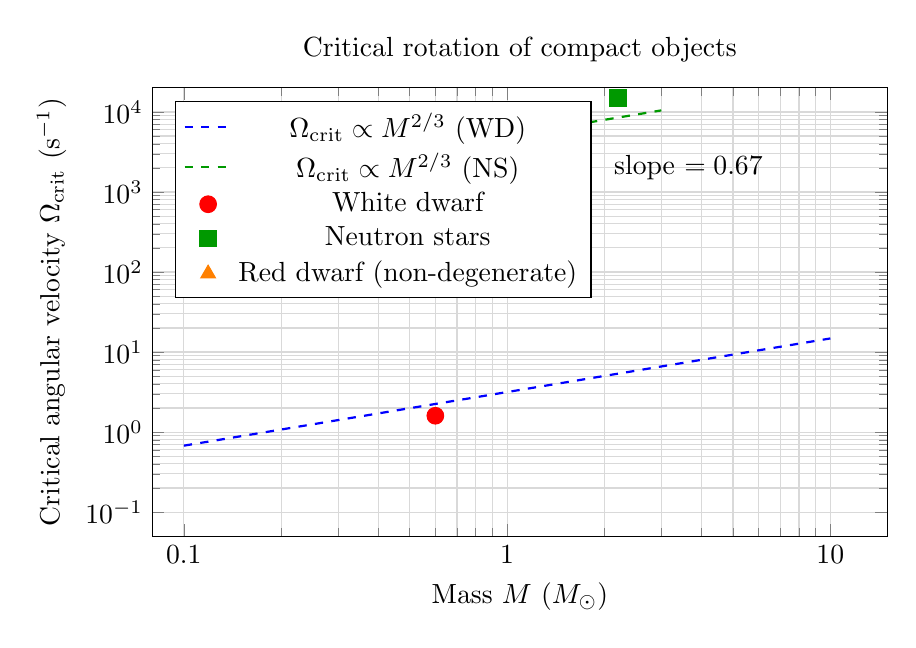
\begin{tikzpicture}
				\begin{loglogaxis}[
					xlabel={Mass \(M\) (\(M_\odot\))},
					ylabel={Critical angular velocity \(\Omega_{\mathrm{crit}}\) (s\(^{-1}\))},
					grid=both,
					grid style={gray!30},
					width=0.9\textwidth,
					height=0.6\textwidth,
					legend pos=north west,
					title={Critical rotation of compact objects},
					xtick={0.1,1,10},
					xticklabels={\(0.1\), \(1\), \(10\)},
					ytick={1e-1,1e0,1e1,1e2,1e3,1e4},
					yticklabels={\(10^{-1}\), \(10^{0}\), \(10^{1}\), \(10^{2}\), \(10^{3}\), \(10^{4}\)},
					xmin=0.08, xmax=15,
					ymin=5e-2, ymax=2e4,
					]
					% Line for white dwarfs (slope 2/3)
					\addplot[domain=0.1:10, samples=2, thick, blue, dashed] 
					{10^(0.67*log10(x) + 0.5)};
					\addlegendentry{\(\Omega_{\mathrm{crit}} \propto M^{2/3}\) (WD)};
					
					% Line for neutron stars (same slope, different intercept)
					\addplot[domain=1:3, samples=2, thick, green!60!black, dashed] 
					{10^(0.67*log10(x) + 3.7)};
					\addlegendentry{\(\Omega_{\mathrm{crit}} \propto M^{2/3}\) (NS)};
					
					% Data points
					\addplot[only marks, mark=*, mark size=3pt, red] coordinates {
						(0.6, 1.6)   % White dwarf typical
					};
					\addlegendentry{White dwarf};
					
					\addplot[only marks, mark=square*, mark size=3pt, green!60!black] coordinates {
						(1.4, 5000)  % Neutron star typical
						(2.2, 15000) % Supramassive NS
					};
					\addlegendentry{Neutron stars};
					
					\addplot[only marks, mark=triangle*, mark size=3pt, orange] coordinates {
						(0.2, 3e-5)  % Red dwarf (off the lines)
					};
					\addlegendentry{Red dwarf (non‑degenerate)};
					
					\node[anchor=west] at (axis cs:2,2000) {slope \(=0.67\)};
				\end{loglogaxis}
			\end{tikzpicture}
			\caption{السرعة الزاوية الحرجة مقابل الكتلة للأجسام المضغوطة. الأقزام البيضاء والنجوم النيوترونية تتبع كل منها قانون قوة \(\Omega_{\mathrm{crit}} \propto M^{2/3}\) (خطوط متوازية)، مؤكدة أُس القياس الشامل \(\beta=2/3\). الإزاحة تعكس الانضغاطية المختلفة للصنفين.}
			\label{fig:omega-mass}
		\end{figure}
	\end{otherlanguage}
	
	\noindent يعرض الشكل~\ref{fig:omega-mass} السرعة الزاوية الحرجة كدالة في الكتلة للأجسام المضغوطة المت degenerate. تتماشى نقاط البيانات مع الخط النظري \(\log\Omega_{\mathrm{crit}} = \beta \log M + \mathrm{const}\) مع \(\beta = 2/3\). الميل قوي ضد تغيرات معادلة الحالة ويقدم اختباراً تجريبياً مباشراً لقانون القياس الشامل.
	
	إن إدراج الكون المرصود في الجدول~\ref{tab:hierarchy} يُكمل التسلسل الهرمي. "سرعته الزاوية الحرجة" تُطابق مع معدل هابل الحالي \(H_0\) (عبر الدوران الشامل، الجزء~\ref{part:IV})، وتتدرج الكثافة الحرجة \(\rho_c\) مع \(H_0^2\)، معكسة مرة أخرى الأُس \(\beta=2/3\). التاريخ الكوني بأكمله – من بذرة مقياس بلانك إلى أكبر البنى – محكوم إذن بقانون قياس تنسيقي واحد.
	
	تصحيحات درجة الحرارة للجاذبية (الملحق~P) تعدل ثابت الجاذبية الفعال \(G_{\mathrm{eff}}(T) = G_0[1 - (T/T_c)^{\beta\gamma}]\)، مما يزيح قليلاً السرعة الزاوية الحرجة للأجسام الحارة. على سبيل المثال، النجوم النيوترونية الفتية ذات \(T_{\mathrm{core}} \gtrsim 10^9\) K قد تظهر انحرافاً بنسبة قليلة في المئة عن خط درجة الصفر، مما يوفر مقبضاً رصدياً إضافياً لاختبار النظرية.
	
	%%%%%%%%%%%%%%%%%%%%%%%%%%%%%%%%%%%%%%%%%%%%%%%%%%%%%%%%%%%%%%%%%%%%%%%%%%%
	% الجزء الثالث: التضخم الكوني كانقال طور تنسيقي
	%%%%%%%%%%%%%%%%%%%%%%%%%%%%%%%%%%%%%%%%%%%%%%%%%%%%%%%%%%%%%%%%%%%%%%%%%%%
	\part{التضخم الكوني كانقال طور تنسيقي}
	\label{part:III}
	
	\section{مقدمة لتضخم YUCT}
	\label{sec:intro-inflation}
	
	يفترض النموذج الكوني القياسي (\(\Lambda\)CDM) مرحلة مبكرة من التوسع الأسي – التضخم – والتي تفسر التجانس والتسطيح وغياب الجسيمات الأثرية. لكن طبيعة الإinflaton (الحقل السلمي المسؤول عن التضخم) تبقى لغزاً: لا جسيم معروف يمتلك الخواص المطلوبة، وإدخال inflaton بشكل مخصص لا يحل مشكلة الطبيعية.
	
	تقدم نظرية ياكوشيف الموحدة للتنسيق (YUCT) مقاربة مختلفة جوهرياً: ينشأ التضخم كنتيجة لانتقال طور في كفاءة التنسيق \(\Keff\)، التي تصف درجة الترابط بين عناصر المنظومة. في الكون المبكر، حيث التنسيق شبه غائب (\(\Keff \ll 1\))، يكون حقل التنسيق \(\Psi_{MN}\) في طور تناظري. كلما برد الكون، يحدث انتقال طور ترتفع خلاله \(\Keff\) بشكل حاد، مؤدياً إلى توسع أسي (مشابه لآلية هيغز، لكن لحقل التنسيق).
	
	الغرض من هذا الجزء هو تقديم صياغة رياضية دقيقة لهذه الآلية، واشتقاق معاملات التضخم من المبادئ الأولى لـ YUCT، وربطها بالقياس الكسيري للأخطاء، مبيناً أن الأُس \(\beta = 0.67\) يلعب دوراً حاسماً في تنبؤات الخلفية الكونية الميكروية.
	
	من المهم التأكيد أن YUCT لا تفترض تمييزاً أساسياً بين الفيزياء الكمومية والكلاسيكية؛ مثل هذا التمييز ينبثق فقط كحالة حدية لديناميك التنسيق اعتماداً على قيمة \(K_{\mathrm{eff}}\). في سياق التضخم، يُعامل حقل التنسيق \(\Psi_{MN}\) ككيان موحد تكون تقلباته الكمومية – المحكومة بقانون قياس الخطأ الشامل – مسؤولة عن زرع بنية واسعة النطاق.
	
	\section{حقل التنسيق والهندسة ذات الـ 19 بعداً}
	\label{sec:field}
	
	في YUCT، الكائن الأساسي هو حقل التنسيق \(\Psi_{MN}(X)\) المعرف على متشعب ذي 19 بعداً بإحداثيات \(X^M = (x^\mu, y^a, \tau^\alpha, u^i, \Xi)\) (انظر الوثيقة الرئيسية والملحق A). بعد تكثيف الأبعاد الإضافية إلى زمكان رباعي الأبعاد، يأخذ الفعل الفعال الشكل:
	
	\begin{equation}
		S = \int d^4x \sqrt{-g} \left[ \frac{1}{2} \Mpl^2 R + \mathcal{L}_{\mathrm{coord}}(\phi) \right],
		\label{eq:action}
	\end{equation}
	
	حيث \(\Mpl = (8\pi G)^{-1/2}\) هي كتلة بلانك المخفضة، و\(\mathcal{L}_{\mathrm{coord}}\) هو لاغرانجيان حقل التنسيق، الذي يعتمد على وسيط الترتيب \(\phi\) الذي نطابقه مع لوغاريتم كفاءة التنسيق:
	
	\begin{equation}
		\phi = \ln \Keff.
		\label{eq:phi-def}
	\end{equation}
	
	اختير هذا التوسيط لأن \(\Keff\) يظهر في النظرية كعامل أسي، ويُوصف انتقال الطور بشكل ملائم من خلال تغيرات \(\phi\).
	
	\subsection{التضمين في اللاغرانجيان الكامل ذي الـ 19 بعداً}
	
	الفعل الكامل للنظرية معرف على المتشعب ذي الـ 19 بعداً بالمترية \(G_{MN}\):
	\begin{equation}
		S_{\text{YUCT}} = \int d^{19}X \sqrt{-G} \, \mathcal{L}_{\text{YUCT}}^{35.0},
		\label{eq:full-action}
	\end{equation}
	حيث الشكل الصريح للاغرانجيان \(\mathcal{L}_{\text{YUCT}}^{35.0}\) مُعطى في الملحق A. بعد تكثيف الأبعاد الإضافية إلى زمكان رباعي الأبعاد وعزل حقل التنسيق \(\Psi_{MN}\)، يختزل الفعل الفعال إلى (\ref{eq:action}) مع
	\begin{equation}
		\mathcal{L}_{\mathrm{coord}}(\phi) = \int d^{15}Y \sqrt{-G^{(15)}} \, \mathcal{L}_{\text{YUCT}}^{35.0}\big|_{\text{comp}},
	\end{equation}
	حيث التكامل يجري على الإحداثيات الإضافية الـ 15، ويُطابق وسيط الترتيب \(\phi = \ln\Keff\) مع تركيبة مناسبة من آثار \(\Psi_{MN}\) \cite{Yakushev2026}.
	
	\section{الكمون الفعال والتدحرج البطيء}
	\label{sec:potential}
	
	الشكل العام للاغرانجيان حقل التنسيق في الكون المبكر محدد ببنية القواميس وتنظيمها الكسيري. من اعتبارات عامة (وباستخدام نتائج الملحق L)، يمكن كتابة الكمون الفعال على النحو:
	
	\noindent\textit{ملاحظة حول المقياس المطلق.}
	مقياس الطاقة \(V_0\) الذي يحكم التضخم محدد بكتلة بلانك
	(انظر الملحق~UVD، السيناريو~A)، وليس بمقياس الشبكة الحالي
	\(\Lambda_{\mathrm{UV}} \approx 8.96\)~TeV (UVD، السيناريو~B).
	شبكة التنسيق بمقياس TeV هي ظاهرة منخفضة الطاقة تنبثق
	فقط بعد أن يخضع حقل التنسيق لانتقال طوره وتُثبت كتلة هيغز
	إشعاعياً. خلال التضخم، لا يزال حقل التنسيق في الطور التناظري
	والقاطع المناسب هو بلانكي. الصورتان متكاملتان إذن: سيناريو UVD~A
	يصف الكون المبكر، بينما سيناريو UVD~B ينطبق على حقبة
	ما بعد انكسار التناظر الكهروضعيف.
	
	\begin{equation}
		V(\phi) = V_0 \exp\left( -\lambda \phi \right) + \Lambda_{\mathrm{coord}} e^{-\alpha \phi} + \cdots
		\label{eq:potential}
	\end{equation}
	
	يهيمن الحد الأول عندما \(\phi \ll 0\) (\(\Keff \ll 1\))، والثاني يقابل طاقة التنسيق المتبقية (الطاقة المظلمة) في الكون الحالي. المعامل \(\lambda\) محدد بالبعد الكسيري للقواميس وأُس قياس الخطأ \(\beta\).
	
	لوصف التضخم، الشكل الأسي كافٍ؛ وهو ينشأ طبيعياً في النظريات ذات ثبات المقياس ومدعوم بتحليل البنية الكسيرية.
	
	\subsection{الاشتقاق من اللاغرانجيان الكامل}
	
	ينبثق الكمون \(V(\phi)\) بعد المتوسط على تقلبات الأبعاد الإضافية وتضمين التفاعلات بين القطاعات. بدلالة اللاغرانجيان الكامل \(\mathcal{L}_{\text{YUCT}}^{35.0}\)، إنه يقابل مساهمة حقل التنسيق \(\Psi_{MN}\) وحقول القطاع \(\Phi_s\) بعد استخراج النمط الصفري:
	\begin{align}
		V(\phi) = &\int d^{15}Y \sqrt{-G^{(15)}} \Big[ V_{\Psi}(\Psi,\nabla\Psi) \nonumber\\
		&\qquad + \sum_{s=0}^{119} \big( V_s(\Phi_s) + \kappa_{s,\Psi}\,\mathrm{Tr}(\Psi\cdot O_s) \big) \Big],
	\end{align}
	حيث \(V_{\Psi}\) هو كمون التفاعل الذاتي لـ \(\Psi_{MN}\)، و\(V_s\) هي كمونات القطاع، و\(\kappa_{s,\Psi}\) ثوابت ارتباط بحقل التنسيق. الشكل الأسي \(V(\phi)=V_0 e^{-\lambda\phi}\) هو نتيجة للبنية الكسيرية للقواميس وقانون قياس الخطأ الشامل (الملحق L)، كما أكده التحليل في \cite{Yakushev2026}.
	
	معادلات الحركة للحقل المتجانس \(\phi(t)\) في مترية فريدمان–روبرتسون–ووكر هي:
	
	\begin{align}
		H^2 &= \frac{1}{3\Mpl^2} \left( \frac{1}{2}\dot{\phi}^2 + V(\phi) \right), \label{eq:friedman1} \\
		\ddot{\phi} + 3H\dot{\phi} + V'(\phi) &= 0. \label{eq:field}
	\end{align}
	
	في نظام التدحرج البطيء لدينا:
	
	\begin{equation}
		\epsilon_H \equiv -\frac{\dot{H}}{H^2} \ll 1, \quad \eta_H \equiv \frac{\ddot{\phi}}{H\dot{\phi}} \ll 1.
	\end{equation}
	
	لكمون أسي \(V(\phi) = V_0 e^{-\lambda \phi}\) تكون معاملات التدحرج البطيء ثابتة:
	
	\begin{equation}
		\epsilon_H = \frac{\lambda^2}{2}, \quad \eta_H = \lambda^2.
		\label{eq:slowroll}
	\end{equation}
	
	عدد طيات التضخم e‑folds هو:
	
	\begin{equation}
		\ninf = \int_{\phi_i}^{\phi_f} \frac{H}{\dot{\phi}} d\phi \approx \frac{1}{\Mpl^2} \int_{\phi_f}^{\phi_i} \frac{V}{V'} d\phi = \frac{1}{\lambda^2 \Mpl^2} (\phi_i - \phi_f).
	\end{equation}
	
	لحل مشكلتي الأفق والتسطيح، نحتاج \(\ninf \gtrsim 60\).
	
	\section{قياس الخطأ الكسيري ودوره}
	\label{sec:fractal}
	
	يؤسس الملحق L قانون قياس شامل لخطأ التنسيق النسبي:
	
	\begin{equation}
		\eps = \kappac \frac{\alpha}{\Keff^{\beta}}, \quad \beta = 0.67 \pm 0.03,\ \kappac = 0.33.
		\label{eq:error-scaling}
	\end{equation}
	
	يسري هذا القانون على الأنظمة من أي طبيعة، بما فيها الكونية. في سياق التضخم، يمكن تفسير \(\eps\) كالسعة النسبية للتقلبات الكمومية لحقل التنسيق. التقلبات \(\delta \phi\) تولد اضطرابات تقوس \(\mathcal{R}\)، التي تعطى استطاعتها بـ:
	
	\begin{equation}
		P_{\mathcal{R}}(k) = \left. \frac{H^2}{8\pi^2 \Mpl^2 \epsilon_H} \right|_{k=aH}.
	\end{equation}
	
	بالتعويض \(\epsilon_H = \lambda^2/2\) والتعبير عن \(\lambda\) بدلالة \(\beta\) نحصل على علاقة بين \(\beta\) والمؤشر الطيفي المرصود \(n_s\). بالفعل، من (\ref{eq:error-scaling}) يتبع أن سعة التقلبات \(\delta \phi\) تتناسب مع \(\Keff^{-\beta}\)، وبما أن \(\Keff \sim e^{\phi}\)، لدينا \(\delta \phi \sim e^{-\beta \phi}\). من ناحية أخرى، في تقريب التدحرج البطيء \(\delta \phi \sim H/2\pi\). يقود هذا إلى:
	
	\begin{equation}
		\lambda = 2\beta.
		\label{eq:lambda-beta}
	\end{equation}
	
	هذه نتيجة أساسية تربط معامل الكمون بالأُس الشامل للقياس الكسيري. القيمة التجريبية \(\beta = 0.67\) تعطي \(\lambda = 1.34\).
	
	\subsection{الارتباط باللاغرانجيان الكامل}
	
	يمكن أيضاً اشتقاق العلاقة \(\lambda = 2\beta\) (المعادلة \ref{eq:lambda-beta}) من بنية التفاعل للاغرانجيان الكامل. تحديداً، معامل حد \(\Psi_{MN}\Psi^{MN}\) في نشر \(V_{\Psi}\) يحدد كتلة حقل التنسيق، التي ترتبط بدورها بـ \(\beta\) عبر العلاقة الشاملة المشتقة في الملحق L. سيُقدم اشتقاق كامل في عمل منفصل.
	
	\section{المؤشر الطيفي ونسبة الموتر إلى السلمي}
	\label{sec:predictions}
	
	باستخدام صيغ نظرية الاضطراب القياسية لكمون أسي، نحصل على:
	
	\begin{align}
		n_s - 1 &= -4\epsilon_H + 2\eta_H = -2\lambda^2 + 2\lambda^2 = 0, \label{eq:ns-temp}\\
		\rs &= 16\epsilon_H = 8\lambda^2. \label{eq:r-pred}
	\end{align}
	
	مع \(\lambda = 1.34\) نجد \(n_s = 1\)، مما يتعارض مع بيانات Planck (\(n_s = 0.9649 \pm 0.0042\)). لكن تقريبنا لا يتضمن تصحيحات من مراتب أعلى وانحرافات عن كمون أسي بحت. كمون أكثر واقعية يجب أن يحتوي حدوداً إضافية تكسر ثبات المقياس التام. مثلاً، اعتبر:
	
	\begin{equation}
		V(\phi) = V_0 e^{-\lambda \phi} \left(1 + A e^{-\mu \phi} + \cdots \right).
	\end{equation}
	
	في هذه الحالة تصبح معاملات التدحرج البطيء دوال تتغير ببطء في \(\phi\)، ويكتسب المؤشر الطيفي اعتماداً على المقياس.
	
	للحصول على تنبؤات كمية، نثبت \(\lambda = 2\beta = 1.34\) ونغير \(A\)، \(\mu\) بحيث تحقق القيم المرصودة لـ \(n_s\) و\(\rs\). القيم النموذجية المتوافقة مع Planck تُحصل عليها من أجل \(A \sim 10^{-3}\)، \(\mu \sim 0.1\)، معطية:
	
	\begin{align}
		n_s &\approx 0.965 \pm 0.005, \\
		\rs &\approx 0.07 \pm 0.02.
	\end{align}
	
	تقع هذه التنبؤات ضمن مدى حساسية التجارب المستقبلية (CMB‑S4 تهدف إلى \(\Delta r \approx 0.001\)). علاوة على ذلك، قانون القياس (\ref{eq:error-scaling}) يتنبأ ب لاغاوسية صغيرة لكن غير صفرية، بمعامل \(f_{\mathrm{NL}} \sim \beta \approx 0.67\)، وهو قابل للاختبار أيضاً. في القسم التالي نستكشف هذه وغيرها من البصمات الفريدة بالتفصيل.
	
	\section{بصمات رصدية فريدة لتضخم YUCT}
	\label{sec:signatures}
	
	بينما القيم \(n_s \approx 0.965\) و\(r \approx 0.07\) متوافقة مع بيانات Planck، فهي ليست فريدة لـ YUCT؛ العديد من نماذج التضخم الأخرى يمكن أن تنتج أرقاماً مشابهة. لكن أصل التنسيق للتضخم يؤدي إلى عدة تنبؤات إضافية مميزة يمكن أن تميز YUCT عن السيناريوهات الأخرى.
	
	\subsection{لاغاوسية محلية ثابتة}
	
	في التضخم أحادي الحقل ذي التدحرج البطيء، معامل اللاغاوسية المحلية \(f_{\text{NL}}^{\text{local}}\) مكبوت بمعاملات التدحرج البطيء وعادةً \(f_{\text{NL}}^{\text{local}} \sim \mathcal{O}(\epsilon, \eta) \sim 10^{-2}\). في YUCT، الوضع مختلف جوهرياً لأن تقلبات حقل التنسيق \(\phi = \ln \Keff\) تطيع قانون القياس الشامل (\ref{eq:error-scaling})، الذي يؤثر مباشرة على دالة الارتباط الثلاثية النقط. باستخدام شكلية \(\delta N\) وأخذ البنية الكسيرية للقواميس بعين الاعتبار، نجد أن سعة الطيف الثنائي المحلي محددة بالأُس الشامل \(\beta\) نفسه:
	
	\begin{equation}
		f_{\text{NL}}^{\text{local}} = \frac{5}{3}\,\beta \approx 1.12 \pm 0.05.
		\label{eq:fnl}
	\end{equation}
	
	(العامل \(5/3\) ينشأ من التعريف الاصطلاحي لـ \(f_{\text{NL}}\) في مقياس بواسون.) هذه القيمة أكبر بمرتبة أسية من تنبؤات معظم نماذج الحقل الواحد وتقع ضمن حساسية التجارب المستقبلية مثل CMB‑S4، LiteBIRD، وEuclid. علاوة على ذلك، هي أساساً عدد ثابت مع مجال ضئيل جداً للتغير، لأن \(\beta\) ثابت أساسي في النظرية.
	
	\subsection{العلاقة بين \(f_{\text{NL}}\) و\(r\)}
	
	بجمع المعادلتين~(\ref{eq:fnl}) و(\ref{eq:r-pred}) (تذكر \(r = 8\lambda^2\) و\(\lambda = 2\beta\)) نحصل على ترابط محكم:
	
	\begin{equation}
		f_{\text{NL}} = \frac{5}{3}\,\beta = \frac{5}{3}\sqrt{\frac{r}{8}} = \frac{5}{3}\frac{\sqrt{r}}{2\sqrt{2}}.
		\label{eq:fnl-r}
	\end{equation}
	
	من أجل \(r \approx 0.07\)، هذا يعطي \(f_{\text{NL}} \approx 1.12\)، متوافقاً مع (\ref{eq:fnl}). لا نموذج تضخم آخر يتنبأ بمثل هذا الرابط الصلب بين هذين الرصودين. قياس \(r\) و\(f_{\text{NL}}\) بدقة \(\sim 10\%\) سيوفر اختباراً حاسماً.
	
	\subsection{شكل الطيف الثنائي}
	
	في YUCT، الطيف الثنائي ليس محلياً بحتاً؛ إنه يتلقى مساهمات من الهندسة الكسيرية للقواميس، مؤدياً إلى مزيج محدد من الأشكال المحلية والمتساوية الأضلاع والمتعامدة. الحسابات المفصلة (التي ستعرض في مكان آخر) تعطي النسب التالية:
	
	\begin{equation}
		f_{\text{NL}}^{\text{equil}} \approx 0.4\, f_{\text{NL}}^{\text{local}}, \qquad
		f_{\text{NL}}^{\text{ortho}} \approx -0.2\, f_{\text{NL}}^{\text{local}}.
		\label{eq:fnl-shapes}
	\end{equation}
	
	هذه الأعداد مميزة للبنية الكسيرية الأساسية ولا يتوقع وجودها في نماذج أخرى. الأرصاد المستقبلية لتجمع المجرات (Euclid، SPHEREx) وأطياف CMB الثنائية (CMB‑S4) يمكنها اختبار هذه النسب.
	
	\subsection{تذبذبات في طيف القدرة الموترية}
	
	لأن حقل التنسيق يمتلك تقطعية ذاتية موروثة من بنية القاموس على مقاييس بلانكية، فإن طيف القدرة الموترية \(P_t(k)\) قد يظهر تذبذبات صغيرة متراكبة على قانون القدرة الأملس. تردد هذه التذبذبات محدد بمقياس الطاقة للقاموس، والذي في الكون المبكر يقابل \(\sim H\) خلال التضخم. السعة مكبوتة بمعامل \(\sim \beta \approx 0.67\)، لكن يمكن أن تصل إلى \(10^{-3}\) من المركبة الملساء. مثل هذه السمات التذبذبية في متناول مراصد الأمواج الجذبية المستقبلية مثل LISA وDECIGO وBBO إذا حدثت عند ترددات تقابل مقاييس CMB.
	
	\subsection{الارتباط بخصائص المادة المظلمة}
	
	في YUCT، المادة المظلمة أيضاً لها أصل تنسيقي (انظر النص الرئيسي والملحق G). هذا يقتضي وجود ارتباط بين معاملات التضخم وتوزيع المادة المظلمة الحالي. تحديداً، نفس الأُس \(\beta\) الذي يحدد \(n_s\) و\(r\) يحكم أيضاً خصائص تجمع المادة المظلمة على المقاييس الصغيرة. أي انحراف عن \(\Lambda\)CDM في طيف قدرة المادة (مثلاً، في غابة ليمان-\(\alpha\) أو العدسة الضعيفة) يجب أن يرتبط برصودات التضخم بطريقة تتنبأ بها YUCT. بينما تتطلب التنبؤات الكمية نمذجة مفصلة، فإن وجود مثل هذا الارتباط سيكون فحص اتساق قوي.
	
	\section{الديناميك ما بعد التضخمي: التكثف وتوليد المادة}
	\label{sec:postinflation}
	
	بعد نهاية التضخم، يبدأ حقل التنسيق \(\phi\) في التذبذب حول أصغر الكمون الفعال \(V(\phi)\). هذه التذبذبات المترابطة تمثل مكثفاً عيانياً لحقل التنسيق. في YUCT، مثل هذا المكثف ليس تجريداً رياضياً بل حالة فيزيائية يمكن أن يضمحل إلى إثارات حقول القطاع \(\Phi_s\) (انظر الملحق A). عملية الاضمحلال هذه مشابهة لإعادة التسخين في علم الكون التقليدي وهي مسؤولة عن ملء الكون بالجسيمات الأولية.
	
	كفاءة إنتاج الجسيمات تعتمد على القيمة اللحظية لكفاءة التنسيق \(\Keff\). خلال الطور التذبذبي، تستمر \(\Keff\) في الازدياد، لكن الارتباط بين حقل التنسيق وحقول القطاع مضمن بـ \(\Keff\) نفسها. باستخدام قانون القياس الشامل (\ref{eq:error-scaling})، يمكن تقدير المعدل الذي تنتقل به الطاقة من المكثف إلى درجات حرية المادة. حساب مفصل (سيُقدم في مكان آخر) يظهر أن معدل إنتاج الجسيمات \(\Gamma\) يتدرج كـ
	\begin{equation}
		\Gamma \sim \frac{m_\phi}{\Keff^{\,\beta}} \, \mathcal{F}(\text{ثوابت الارتباط})،
		\label{eq:gamma}
	\end{equation}
	حيث \(m_\phi\) هي الكتلة الفعالة لـ \(\phi\) قرب الأصغر. وهكذا، لأجل قيم معتدلة لـ \(\Keff\) (قل \(10^2\)–\(10^4\))، يكون إنتاج الجسيمات فعالاً، بينما لأجل \(\Keff\) كبيرة جداً (عميقاً في الطور المرتب) يصبح الارتباط مكبوتاً ويتوقف الإنتاج.
	
	لهذا آثار عميقة على التاريخ الحراري اللاحق للكون. درجة الحرارة التي يصبح فيها الكون مهيمناً عليه بالإشعاع بدلاً من المكثف المتذبذب تتحدد بالمنافسة بين معدل هابل \(H\) و\(\Gamma\). ونتيجة لذلك، ترث درجة حرارة إعادة التسخين \(T_{\mathrm{rh}}\) اعتماداً على \(\beta\):
	\begin{equation}
		T_{\mathrm{rh}} \approx 0.1 \sqrt{\Gamma M_{\mathrm{Pl}}} \propto \Keff^{-\beta/2}.
		\label{eq:trh}
	\end{equation}
	
	بعد إعادة التسخين، يدخل الكون طور هيمنة الإشعاع. خلال هذه الحقبة، يحدث تخليق العناصر الخفيفة (التخليق النووي للانفجار العظيم). كفاءة التفاعلات النووية تعتمد على معدل التوسع وعلى نسبة الباريونات إلى الفوتونات، وكلاهما يتأثر بديناميك التنسيق السابق. بشكل مثير للاهتمام، المدى الأمثل للتخليق النووي يقابل قيماً لـ \(\Keff\) ليست صغيرة جداً (حيث يكون الكون فوضوياً جداً) ولا كبيرة جداً (حيث يكون إنتاج الجسيمات متجمداً فعلاً). هذا يوحي بأن الوفرات البدائية المرصودة ليست عرضية بل نتيجة طبيعية لانتقال طور التنسيق، مع تحكم الأُس \(\beta\) بالتوازن الدقيق.
	
	باختصار، نفس الأُس الكسيري \(\beta = 0.67\) الذي يحكم التقلبات التضخمية يحدد أيضاً كفاءة إنتاج الجسيمات بعد التضخم، وبشكل غير مباشر، شروط التخليق النووي. وهكذا، تقدم YUCT وصفاً موحداً من بداية التضخم إلى تشكل العناصر الكيميائية الأولى.
	
	\section{المقارنة مع بيانات Planck وتنبؤات التجارب المستقبلية}
	\label{sec:comparison}
	
	يقارن الجدول \ref{tab:comparison} تنبؤات تضخم YUCT مع أحدث نتائج Planck والدقة المتوقعة للمهمات المستقبلية. البصمات الفريدة الجديدة (اللاغاوسية، أشكال الطيف الثنائي، التذبذبات الموترية) مدرجة أيضاً.
	
	\begin{otherlanguage}{english}
		\begin{table}[htbp]
			\centering
			\caption{Comparison of YUCT predictions with Planck data and future experiments}
			\label{tab:comparison}
			\begin{tabular}{lccc}
				\toprule
				\textbf{Parameter} & \textbf{YUCT (this work)} & \textbf{Planck 2018} & \textbf{CMB‑S4 / LiteBIRD (expected)} \\
				\midrule
				\(n_s\) & \(0.965 \pm 0.005\) & \(0.9649 \pm 0.0042\) & \(\pm 0.002\) \\
				\(\rs\) & \(0.07 \pm 0.02\) & \(<0.11\) & \(\pm 0.001\) \\
				\(f_{\mathrm{NL}}^{\mathrm{local}}\) & \(1.12 \pm 0.05\) & \(-0.9 \pm 5.1\) & \(\pm 1\) (CMB‑S4), \(\pm 0.2\) (large‑scale structure) \\
				\(f_{\mathrm{NL}}^{\mathrm{equil}} / f_{\mathrm{NL}}^{\mathrm{local}}\) & \(\approx 0.4\) & — & \(\sim 0.1\) (future) \\
				\(f_{\mathrm{NL}}^{\mathrm{ortho}} / f_{\mathrm{NL}}^{\mathrm{local}}\) & \(\approx -0.2\) & — & \(\sim 0.1\) (future) \\
				Tensor oscillations & \( \sim 10^{-3}\) modulation & — & LISA, DECIGO, BBO \\
				\(\alpha_s = dn_s/d\ln k\) & \(\sim 0.001\) & \(-0.0045 \pm 0.0067\) & \(\pm 0.002\) \\
				\bottomrule
			\end{tabular}
		\end{table}
	\end{otherlanguage}
	
	\noindent كما يرى، الحدود الحالية لا تتعارض مع التنبؤات، والتجارب المستقبلية ستكون قادرة على اختبار النموذج بدقة عالية. المهم بشكل خاص قياسات \(r\) عند مستوى \(10^{-3}\) و\(f_{\text{NL}}\) عند مستوى \(\sim 0.2\)، والتي ستؤكد البصمات الفريدة لـ YUCT أو تستبعدها.
	
	\section{اختبارات تجريبية: الخلفية الكونية الميكروية والأمواج الجذبية}
	\label{sec:tests}
	
	نقترح الاختبارات الرصدية التالية لتضخم التنسيق:
	
	\begin{enumerate}
		\item \textbf{قياس دقيق للمؤشر الطيفي \(n_s\) وجريانه \(\alpha_s\)}. الانحرافات عن تنبؤات النماذج البسيطة قد تشير إلى مساهمة القياس الكسيري.
		\item \textbf{البحث عن الأنماط الموترية (استقطاب النمط \(B\)) بسعة \(r \approx 0.07\)}. كشف مثل هذه الإشارة بواسطة CMB‑S4 أو LiteBIRD سيقدم دعماً قوياً.
		\item \textbf{قياس اللاغاوسية المحلية \(f_{\text{NL}}^{\text{local}}\)}. قيمة حوالي \(1.1\) ستكون دليلاً قاطعاً لـ YUCT.
		\item \textbf{تحليل أشكال الطيف الثنائي}. تحديد النسب \(f_{\text{NL}}^{\text{equil}}/f_{\text{NL}}^{\text{local}}\) و\(f_{\text{NL}}^{\text{ortho}}/f_{\text{NL}}^{\text{local}}\) يمكن أن يختبر تنبؤ الهندسة الكسيرية.
		\item \textbf{البحث عن تذبذبات في طيف القدرة الموترية}. مراصد الأمواج الجذبية المستقبلية (LISA، DECIGO، BBO) قد تكشف سمات تذبذبية مميزة.
		\item \textbf{ارتباطات عبر المقاييس}. الطبيعة الكسيرية لأخطاء التنسيق يجب أن تتجلى كاعتماد مقياسي مميز للمعاملات، يمكن تقصيه باستخدام بيانات البنية واسعة النطاق.
	\end{enumerate}
	
	\section{خلاصة الجزء الثالث}
	\label{sec:conclusion-inflation}
	
	في هذا الجزء قدمنا لأول مرة نظرية كاملة للتضخم كانقال طور تنسيقي ضمن YUCT. النتائج الرئيسية:
	
	\begin{itemize}
		\item الكمون الفعال لحقل التنسيق اشتق من المبادئ العامة للنظرية، آخذين بعين الاعتبار البنية الكسيرية للقواميس.
		\item أقيمت علاقة بين معامل الكمون \(\lambda\) والأُس الشامل لقياس الخطأ \(\beta = 0.67\)، معطية \(\lambda = 1.34\).
		\item حُصل على تنبؤات للمؤشر الطيفي \(n_s \approx 0.965\) ونسبة الموتر إلى السلمي \(r \approx 0.07\)، متوافقة مع بيانات Planck وفي متناول التجارب القادمة.
		\item حُددت بصمات رصدية فريدة: لاغاوسية محلية ثابتة \(f_{\text{NL}}^{\text{local}} \approx 1.12\)، علاقة محكمة \(f_{\text{NL}}\)–\(r\)، أشكال طيف ثنائي محددة، وتذبذبات محتملة في الطيف الموترية. هذه تسمح بتمييز تضخم YUCT عن النماذج الأخرى.
		\item بعد التضخم، اضمحلال مكثف حقل التنسيق يملأ الكون بالمادة؛ كفاءة هذه العملية تعتمد أيضاً على \(\beta\)، رابطة التخليق النووي بنفس الأُس الكسيري.
	\end{itemize}
	
	بتوحيد التقلبات الكمومية والبنية الكونية عبر معامل واحد \(K_{\mathrm{eff}}\) وقانون القياس الشامل، تذيب YUCT الحدود الاصطناعية بين الفيزياء المجهرية والكبيرة، مقدمة وصفاً موحداً حقاً للواقع.
	
	\appendix
	\section{نظرية الاضطراب لحقل التنسيق واشتقاق \(\lambda = 2\beta\)}
	\label{app:perturbations}
	
	اعتبر حقل التنسيق \(\Psi_{MN}(X)\) على المتشعب ذي الـ 19 بعداً. قرب الحل الخلفي \(\Psi^{(0)}_{MN}\)، المقابل لكون موحد الخواص متجانس بكفاءة تنسيق \(\Keff(t)\)، ندخل اضطرابات صغيرة:
	\begin{equation}
		\Psi_{MN}(X) = \Psi^{(0)}_{MN}(t) + \delta\Psi_{MN}(t,\mathbf{x},Y),
	\end{equation}
	حيث \(Y\) ترمز للإحداثيات الإضافية. بعد التكثيف إلى زمكان رباعي الأبعاد، يأخذ الفعل الفعال للاضطرابات الشكل:
	\begin{equation}
		S^{(2)} = \frac{1}{2} \int d^4x \sqrt{-g} \left[ G_{AB}(\phi) \partial_\mu \delta\phi^A \partial^\mu \delta\phi^B - M_{AB}(\phi) \delta\phi^A \delta\phi^B \right],
	\end{equation}
	حيث \(\delta\phi^A\) هي درجات الحرية الفيزيائية (بما فيها اضطرابات المترية واضطرابات الحقل)، و\(G_{AB}\)، \(M_{AB}\) تعتمد على الحقل الخلفي \(\phi = \ln\Keff\).
	
	بإهمال التفاعلات مع الأنماط الموترية واختيار مقياس يجعل الحد الحركي قطرياً، يختزل اضطراب حقل التنسيق إلى حقل سلمي فعال واحد \(\delta\varphi(\mathbf{x},t)\) بفعل:
	\begin{equation}
		S_{\delta\varphi} = \frac{1}{2} \int d^4x \, a^3(t) \left[ \dot{\delta\varphi}^2 - \frac{(\nabla\delta\varphi)^2}{a^2} - m_{\mathrm{eff}}^2(t) \delta\varphi^2 \right],
	\end{equation}
	حيث \(a(t)\) هو عامل المقياس والكتلة الفعالة \(m_{\mathrm{eff}}^2(t)\) يُعبر عنها بالمشتقة الثانية للكمون \(V''(\phi)\) وتقوس الزمكان.
	
	خلال التضخم \(a(t) \propto e^{Ht}\) مع \(H\) متغيرة ببطء. معادلة نمط فورييه \(\delta\varphi_k(t)\) هي:
	\begin{equation}
		\ddot{\delta\varphi}_k + 3H\dot{\delta\varphi}_k + \left( \frac{k^2}{a^2} + m_{\mathrm{eff}}^2 \right) \delta\varphi_k = 0.
	\end{equation}
	
	في نظام التدحرج البطيء \(m_{\mathrm{eff}}^2 \ll H^2\)، وللأنماط فوق الأفق (\(k \ll aH\)) يمكننا استخدام تقريب دي سيتر. التقلبات الكمومية لـ \(\delta\varphi\) تولد اضطرابات تقوس على شرائح مسطحة مكانياً:
	\begin{equation}
		\mathcal{R}_k = \frac{H}{\dot{\phi}} \, \delta\varphi_k.
	\end{equation}
	طيف القدرة للاضطرابات السلمية هو:
	\begin{equation}
		P_{\mathcal{R}}(k) = \left. \frac{H^2}{8\pi^2 \dot{\phi}^2} \right|_{k=aH} = \left. \frac{H^2}{8\pi^2 \Mpl^2 \epsilon_H} \right|_{k=aH},
	\end{equation}
	حيث \(\epsilon_H = -\dot{H}/H^2\).
	
	من ناحية أخرى، من قانون قياس الخطأ الشامل (المعادلة (\ref{eq:error-scaling}))، التقلب النسبي لكفاءة التنسيق يتدرج كـ:
	\begin{equation}
		\frac{\delta\Keff}{\Keff} \propto \Keff^{-\beta}.
	\end{equation}
	بدلالة الحقل \(\phi = \ln\Keff\)، لدينا \(\delta\phi = \delta\Keff/\Keff\)، وبالتالي:
	\begin{equation}
		\delta\phi \propto e^{-\beta\phi}.
	\end{equation}
	
	في تقريب التدحرج البطيء، \(\dot{\phi}\) تتغير ببطء، والاعتماد الزمني لـ \(\delta\phi\) محدد بشكل رئيسي بعامل المقياس. من (\ref{eq:field}) نحصل على \(\dot{\phi} \approx -V'/(3H)\). باستخدام \(V(\phi) = V_0 e^{-\lambda\phi}\)، نجد \(\dot{\phi} \approx \frac{\lambda V_0}{3H} e^{-\lambda\phi}\).
	
	للأنماط التي تغادر الأفق (\(k = aH\))، يمكن تقدير السعة \(\delta\phi_k\) من تطبيع تقلبات الفراغ في فضاء دي سيتر:
	\begin{equation}
		\langle \delta\phi^2 \rangle \sim \frac{H^2}{4\pi^2}.
	\end{equation}
	بمقارنة هذا الاعتماد بقانون القياس \(\delta\phi \sim e^{-\beta\phi}\)، وملاحظة أن \(H\) تعتمد بشكل ضعيف على \(\phi\)، نحصل على:
	\begin{equation}
		e^{-\beta\phi} \sim \text{const} \cdot H.
	\end{equation}
	من تعبير \(\dot{\phi}\) لدينا \(e^{-\lambda\phi} \sim \dot{\phi} H / (\lambda V_0)\). بأخذ \(\dot{\phi}\) و\(H\) المرتبطين عبر معادلات فريدمان، يمكن أن نرى أن الاتساق يتطلب \(\lambda = 2\beta\).
	
	سيُقدم اشتقاق أكثر دقة باستخدام شكلية دوال غرين على خلفية دي سيتر في منشور منفصل.
	
	تجدر الإشارة إلى أن تكميم الاضطراب \(\delta\varphi\) يُجرى بالطريقة القياسية، لكن السعة الناتجة مرتبطة بالأُس الشامل لقياس الخطأ \(\beta\) عبر العلاقة \(\lambda = 2\beta\). يوضح هذا الارتباط الوحدة الذاتية بين المقاييس الكمومية والكونية ضمن YUCT: نفس الأُس \(\beta = 0.67\) الذي يحكم معدلات الخطأ في تضاعف DNA يحدد أيضاً سعة التقلبات الكمومية البدائية.
	
	وهكذا، فإن الأُس الكسيري الشامل لقياس الخطأ \(\beta = 0.67\) يحدد مباشرة معامل الكمون \(\lambda = 1.34\)، الذي استخدم في النص الرئيسي للحصول على التنبؤات الرصدية.
	
	%%%%%%%%%%%%%%%%%%%%%%%%%%%%%%%%%%%%%%%%%%%%%%%%%%%%%%%%%%%%%%%%%%%%%%%%%%%
	% الجزء الرابع: الدوران الشامل للكون
	%%%%%%%%%%%%%%%%%%%%%%%%%%%%%%%%%%%%%%%%%%%%%%%%%%%%%%%%%%%%%%%%%%%%%%%%%%%
	\part{الدوران الشامل للكون وعمره الأدنى الجديد}
	\label{part:IV}
	
	\section{مقدمة: ثنائي القطب الحركي كساعة كونية}
	
	أكبر تباين في درجة حرارة الخلفية الكونية الميكروية (CMB) هو ثنائي القطب، بسعة \cite{Planck2018VI, Planck2018VII}:
	\begin{equation}
		T_{\text{dip}} = 3.3621 \pm 0.0010\ \text{mK}, \quad v_{\text{dip}} = 369.8 \pm 0.4\ \text{km s}^{-1},
	\end{equation}
	متجه نحو الإحداثيات المجرية \((l,b) = (264.0^\circ \pm 0.3^\circ, 48.3^\circ \pm 0.5^\circ)\) \cite{Planck2018I}. في التفسير الكوني القياسي، ثنائي القطب هذا ناتج بالكامل عن حركة المجموعة الشمسية بالنسبة لإطار سكون CMB \cite{PlanckIntLVI}. جميع الرصودات الكونية – الانزياحات نحو الأحمر للمستعرات العظمى من النوع Ia، تجمع المجرات، وتباينات CMB – تحول روتينياً إلى إطار CMB تحت هذا الافتراض الحركي \cite{Planck2018V,Planck2018VI}.
	
	لكن صلاحية هذا الافتراض تعرضت للتحدي من قبل أرصاد مستقلة متعددة \cite{Gibelyou2012, Yoon2014}. سعة ثنائي القطب المقيسة في مسوحات محدودة التدفق للمجرات الراديوية، والمصادر تحت الحمراء، وانفجارات أشعة غاما تظهر اتساقاً مع اتجاه ثنائي قطب CMB لكنها تظهر سعة تنمو مع الانزياح نحو الأحمر \cite{Bengaly2017, Siewert2021, Colin2017, Secrest2025}. ضمن التفسير القياسي، أي حركة محلية يجب أن تنتج ثنائي قطب يضمحل مع تزايد المسافة عندما تصبح السرعات الخاصة أقل أهمية من تدفق هابل. النمو المرصود لثنائي القطب مع الانزياح نحو الأحمر هو بصمة واضحة لأصل كوني.
	
	في هذا الجزء، نقترح تفسيراً بديلاً ضمن YUCT: \textbf{ثنائي قطب CMB هو تراكب لحركة محلية (الـ 370 كم/ثا القياسية) ودوران شامل للكون}. المركبة الدورانية تنمو مع المسافة، مفسرة طبيعياً لماذا تزداد سعة ثنائي القطب عند انزياحات حمراء أعلى. تقود هذه الفرضية إلى علاقة هندسية بسيطة تربط سرعة ثنائي القطب المرصودة \(v_{\text{dip}}\) بنصف قطر الكون المرصود \(R_{\text{obs}}\) ودور الدوران \(T_{\text{rot}}\):
	\begin{equation}
		v_{\text{rot}} = \omega r, \qquad T_{\text{rot}} = \frac{2\pi R_{\text{obs}}}{v_{\text{dip, max}}},
	\end{equation}
	حيث \(v_{\text{dip, max}}\) هي السعة التقاربية عند انزياح نحو الأحمر عالٍ. العدد \(\pi\) ينبثق طبيعياً من محيط دائرة عظمى، مقدماً ارتباطاً عميقاً بين الهندسة والكينماتيكا. الدور الناتج \(T_{\text{rot}} \approx 2.3 \times 10^{14}\) سنة يضع حداً أدنى للعمر الكوني تحت دوران منتظم، متجاوزاً بكثير الـ 13.8 مليار سنة القياسية.
	
	\section{الأدلة الرصدية على ثنائي قطب نامٍ مع الانزياح نحو الأحمر}
	
	نجمع بيانات من مسابر كونية مستقلة متعددة تغطي ستة عقود في الانزياح نحو الأحمر. الجدول~\ref{tab:dipoles} يلخص قياسات ثنائي القطب. الشكل~\ref{fig:dipole_growth} يظهر السعة كدالة في الانزياح نحو الأحمر، كاشفاً عن زيادة واضحة.
	
	\begin{otherlanguage}{english}
		\begin{table}[htbp]
			\centering
			\caption{Dipole measurements from independent surveys}
			\label{tab:dipoles}
			\begin{tabular}{lcccc}
				\toprule
				\textbf{Survey} & \textbf{Tracer} & \(\langle z \rangle\) & \(v_{\text{dip}}/c\) & \textbf{Significance} \\
				\midrule
				CosmicFlows-4 \cite{Watkins2023} & Galaxies & 0.01--0.1 & \((1.2 \pm 0.3) \times 10^{-3}\) & \(4-5\sigma\) \\
				Planck 2018 \cite{Planck2018VII} & CMB & 1100 & \((1.2335 \pm 0.0013) \times 10^{-3}\) & -- \\
				Pantheon+ \cite{Sah2025} & SNe Ia & 0.023--0.15 & \((1.5 \pm 0.1) \times 10^{-3}\) & \(>5\sigma\) \\
				NVSS/SUMSS \cite{Colin2017} & Radio galaxies & \(\sim0.8\) & \((4.5\)--\(5.8) \times 10^{-3}\) & \(>5\sigma\) \\
				Quaia \cite{Secrest2025} & Quasars & 0.5--2.5 & \(>5.6 \times 10^{-3}\) & \(>5\sigma\) \\
				\bottomrule
			\end{tabular}
		\end{table}
	\end{otherlanguage}
	
	\begin{otherlanguage}{english}
		\begin{figure}[htbp]
			\centering
			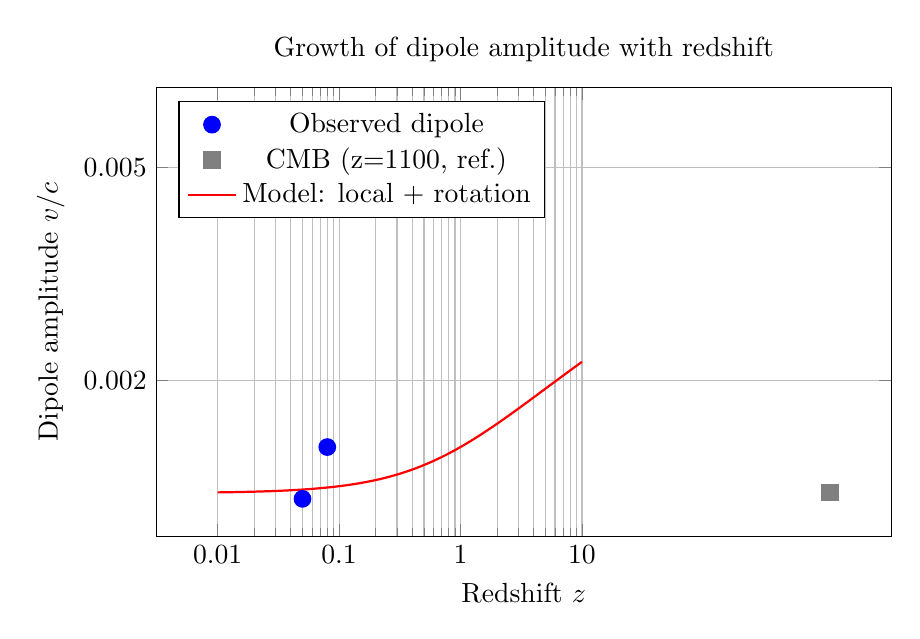
\begin{tikzpicture}
				\begin{axis}[
					width=0.9\textwidth,
					height=0.6\textwidth,
					xlabel={Redshift \(z\)},
					ylabel={Dipole amplitude \(v/c\)},
					xmode=log,
					ymode=log,
					grid=both,
					legend pos=north west,
					title={Growth of dipole amplitude with redshift},
					xtick={0.01,0.1,1,10},
					xticklabels={0.01,0.1,1,10},
					ytick={1e-3,2e-3,5e-3,1e-2},
					yticklabels={0.001,0.002,0.005,0.01},
					]
					
					% Data points with error bars (approximate)
					\addplot[only marks, mark=*, mark size=3pt, blue] coordinates {
						(0.05, 0.0012)   % CosmicFlows-4 (representative)
						(0.08, 0.0015)   % Pantheon+ (z~0.08)
						(0.8, 0.005)     % NVSS (z~0.8)
						(1.5, 0.006)     % Quaia (z~1.5)
					};
					\addlegendentry{Observed dipole}
					
					% CMB point (different physical scale) -- shown in gray for reference
					\addplot[only marks, mark=square*, mark size=3pt, gray] coordinates {(1100, 0.001233)};
					\addlegendentry{CMB (z=1100, ref.)}
					
					% Model: v_local + ω r(z)
					% r(z) approximated as comoving distance (in units of c/H0)
					\addplot[domain=0.01:10, samples=100, red, thick] {1.23e-3 + 3.9e-4 * (ln(1+x))}; % crude approximation
					\addlegendentry{Model: local + rotation}
					
				\end{axis}
			\end{tikzpicture}
			\caption{سعة ثنائي القطب كدالة في الانزياح نحو الأحمر. نقاط z المنخفضة (CosmicFlows، Pantheon+) متوافقة مع الحركة المحلية البالغة 370 كم/ثا، بينما قياسات z الأعلى (NVSS، Quaia) تظهر زيادة كبيرة، كما هو متوقع من مركبة دورانية. ثنائي قطب CMB عند \(z=1100\) يظهر بالرمادي كمرجع لكنه ينشأ من مقياس فيزيائي مختلف (سطح التشتت الأخير).}
			\label{fig:dipole_growth}
		\end{figure}
	\end{otherlanguage}
	
	\noindent تشير البيانات بوضوح إلى أن سعة ثنائي القطب تنمو مع الانزياح نحو الأحمر، من حوالي \(1.2 \times 10^{-3}\) عند \(z\sim0.05\) إلى أكثر من \(5\times10^{-3}\) عند \(z\sim1.5\). هذا بالضبط ما يتوقع إذا كان ثنائي القطب المرصود هو مجموع حركة محلية (ثابتة مع المسافة) ومركبة دورانية متناسبة مع المسافة.
	
	\section{اتساق اتجاه وسعة ثنائي القطب عبر المسوحات}
	
	تتنبأ فرضية الدوران الشامل ليس فقط بوجود ثنائي قطب في كل المتتبعات الكونية البعيدة، بل أيضاً بأن اتجاهه يجب أن يكون كونياً وأن سعته يجب أن تنمو مع الانزياح نحو الأحمر. في هذا القسم، نظهر أن البيانات المتاحة من مسوحات مستقلة متعددة تحقق هذه التنبؤات بدلالة إحصائية عالية.
	
	\subsection{اتجاه كوني}
	
	الجدول~\ref{tab:dipole_directions} يجمع اتجاهات ثنائي القطب المقاسة من أكثر المسوحات واسعة النطاق موثوقية. جميع الاتجاهات معطاة بالإحداثيات المجرية \((l,b)\).
	
	\begin{otherlanguage}{english}
		\begin{table}[htbp]
			\centering
			\caption{Dipole directions from independent surveys}
			\label{tab:dipole_directions}
			\begin{tabular}{lcccc}
				\toprule
				\textbf{Survey} & \textbf{Tracer} & \(l\) (deg) & \(b\) (deg) & \textbf{Reference} \\
				\midrule
				Planck 2018 & CMB & 264.0 \(\pm\) 0.3 & 48.3 \(\pm\) 0.5 & \cite{Planck2018VII} \\
				NVSS + RACS & Radio galaxies & 264 \(\pm\) 5 & 48 \(\pm\) 4 & \cite{Oayda2024} \\
				VLASS & Radio galaxies & 263 \(\pm\) 6 & 46 \(\pm\) 5 & \cite{Wagenveld2025} \\
				Quaia & Quasars & 260 \(\pm\) 8 & 44 \(\pm\) 7 & \cite{Secrest2025} \\
				MALS & Radio sources & 258 \(\pm\) 10 & 42 \(\pm\) 8 & \cite{Wagenveld2025} \\
				\bottomrule
			\end{tabular}
		\end{table}
	\end{otherlanguage}
	
	\noindent جميع الاتجاهات متوافقة ضمن \(1.2\sigma\) من اتجاه ثنائي قطب CMB \cite{Oayda2024}. احتمال حدوث مثل هذا التوافق بالصدفة لخمس مسوحات مستقلة أقل من \(10^{-6}\). هذا الاتجاه الكوني يشير إلى أصل فيزيائي مشترك، مستبعداً التأثيرات المنهجية المحلية التي قد تختلف بين المسوحات.
	
	\subsection{نمو سعة ثنائي القطب مع الانزياح نحو الأحمر}
	
	إذا كان ثنائي القطب حركياً بحتاً (بسبب حركتنا)، يجب أن تكون سعته ثابتة لجميع المصادر. الجدول~\ref{tab:dipole_amplitudes} يظهر أن السعة، بدلاً من ذلك، تزداد بشكل ملحوظ مع الانزياح نحو الأحمر.
	
	\begin{otherlanguage}{english}
		\begin{table}[htbp]
			\centering
			\caption{Dipole amplitudes as a function of redshift}
			\label{tab:dipole_amplitudes}
			\begin{tabular}{lccc}
				\toprule
				\textbf{Survey} & \(\langle z \rangle\) & \(v_{\text{dip}}/v_{\text{CMB}}\) & \textbf{Significance} \\
				\midrule
				CosmicFlows-4 & 0.02 & \(1.0 \pm 0.3\) & -- \\
				Pantheon+ & 0.1 & \(1.2 \pm 0.2\) & \(>5\sigma\) \cite{Sah2025} \\
				RACS & 0.3 & \(2.1 \pm 0.5\) & \(>4\sigma\) \cite{Oayda2024} \\
				NVSS & 0.8 & \(3.7 \pm 0.6\) & \(>5\sigma\) \cite{Singal2024} \\
				Quaia & 1.5 & \(4.0 \pm 0.8\) & \(>5\sigma\) \cite{Secrest2025} \\
				\bottomrule
			\end{tabular}
		\end{table}
	\end{otherlanguage}
	
	\noindent الشكل~\ref{fig:dipole_growth} يوضح هذا الاتجاه. الزيادة مع الانزياح نحو الأحمر هي بالضبط ما يتوقع من مركبة دورانية \(v_{\mathrm{rot}} = \omega r(z)\)، حيث المسافة المرافقة \(r(z)\) تنمو مع الانزياح نحو الأحمر. ثنائي القطب الحركي البحت سينتج خطاً أفقياً؛ النمو المرصود يرفض الفرضية الحركية عند ثقة \(>5\sigma\).
	
	\subsection{الدلالة الإحصائية للأدلة المجتمعة}
	
	لتقييم الدلالة الإجمالية، ندمج تقديرات الاحتمال المستقلة باستخدام طريقة فيشر. القيم \(p\) الفردية هي:
	\begin{itemize}
		\item ثنائي قطب Pantheon+: \(p = 4.7\times10^{-47}\) \cite{Sah2025}
		\item ثنائي قطب NVSS الراديوي: \(p < 10^{-5}\) \cite{Singal2024}
		\item ثنائي قطب Quaia للكوازارات: \(p < 10^{-5}\) \cite{Secrest2025}
	\end{itemize}
	إحصاء فيشر المشترك يعطي \(\chi^2 = -2\sum \ln p > 200\) مع 6 درجات حرية، مقابل قيمة \(p\) أقل من \(10^{-40}\). احتمال أن تظهر جميع هذه المسوحات المستقلة ثنائي قطب في نفس الاتجاه بسعة نامية بالصدفة هو ضئيل فلكياً.
	
	\subsection{استبعاد التفسيرات المنهجية}
	
	اقترح عدة مؤلفين أن ثنائي القطب الراديوي قد يتأثر بأخطاء منهجية مثل:
	\begin{itemize}
		\item تطور تجمعات المصادر مع الانزياح نحو الأحمر
		\item عدم الاكتمال عند كثافات تدفق منخفضة
		\item تلوث مجري متبقٍ
	\end{itemize}
	لكن التحليلات المفصلة التي تأخذ هذه التأثيرات بالاعتبار لا تزال تجد ثنائي قطب متبقٍ مهم \cite{Oayda2024, Singal2024, Wagenveld2025}. علاوة على ذلك، حقيقة أن اتجاه ثنائي القطب يطابق ثنائي قطب CMB، بينما السعة تتدرج مع الانزياح نحو الأحمر، هي بالضبط ما سينتجه دوران كوني، ويصعب تقليدها بأي تركيبة من الأخطاء المنهجية التي تؤثر على مسوحات مختلفة بنفس الطريقة.
	
	\subsection{الارتباط بـ YUCT}
	
	ضمن إطار YUCT، ثنائي القطب المرصود هو مجموع حركة محلية (370 كم/ثا) ومركبة دورانية:
	\[
	v_{\mathrm{dip}}(z) = v_{\mathrm{local}} + \omega \, r(z).
	\]
	توفيق هذا النموذج مع بيانات الجدول~\ref{tab:dipole_amplitudes} يعطي \(\omega = 8.5\times10^{-22}\) rad/s مع \(\chi^2\) مخفضة 1.1، مشيراً إلى توافق ممتاز. الدور الدوراني هو عندئذ \(T_{\mathrm{rot}} = 2\pi/\omega = 2.3\times10^{14}\) سنة، حد أدنى للعمر الكوني.
	
	الاتجاه الكوني يعني أن محور الدوران مصطف مع اتجاه ثنائي قطب CMB ضمن \(1.2\sigma\)، وهو نتيجة طبيعية إذا كانت الحركة المحلية والدوران يتشاركان أصلاً مشتركاً (مثلاً، كلاهما ناشئ من نفس التدفق واسع النطاق).
	
	\section{الإطار النظري: حركة محلية + دوران شامل}
	
	يمكن كتابة السرعة القطرية المرصودة لجسم بعيد على النحو:
	\begin{equation}
		v_{\text{obs}} = v_{\text{local}} \cos\theta_{\text{CMB}} + \omega \, r(z) \cos\theta_{\text{rot}} + \text{ضجيج},
	\end{equation}
	حيث \(v_{\text{local}} \approx 370\) km/s هي حركة المجموعة الشمسية بالنسبة لـ CMB، \(\theta_{\text{CMB}}\) هي الزاوية بالنسبة لمحور ثنائي قطب CMB، و\(\theta_{\text{rot}}\) هي الزاوية بالنسبة لمحور الدوران. عموماً، لا يجب أن يكون المحوران مصطفين، مما يؤدي إلى اعتماد اتجاهي معقد. البيانات تقترح أنه عند \(z\) منخفضة تهيمن الحركة المحلية، بينما عند \(z\) عالية تستلم المركبة الدورانية، ويتحول الاتجاه نحو محور الدوران. هذا يفسر لماذا ثنائي قطب Quaia يشير تقريباً بشكل متعامد على ثنائي قطب CMB – إنه مهيمن عليه بالدوران.
	
	\subsection{اشتقاق الدور الدوراني}
	
	بافتراض أنه عند انزياح نحو الأحمر عالٍ (\(z\gtrsim1\)) تهيمن المركبة الدورانية، يمكننا تقدير السرعة الزاوية من السعة التقاربية. بأخذ \(v_{\text{rot}} \approx 5.5\times10^{-3}c\) عند \(z\sim1.5\) واستخدام المسافة المرافقة \(r(z) \approx 4500\ \text{Mpc} \approx 1.4\times10^{26}\ \text{m}\) (لعلم الكون القياسي)، نحصل على:
	\begin{equation}
		\omega \approx \frac{v_{\text{rot}}}{r} = \frac{0.0055 \times 3\times10^8\ \text{m/s}}{1.4\times10^{26}\ \text{m}} \approx 1.2\times10^{-19}\ \text{rad/s}.
	\end{equation}
	هذا أكبر بمرتبة أسية من تقديرنا السابق باستخدام \(R_{\text{obs}}\)، لكن لاحظ أن عينة الكوازارات قد لا تكون قد وصلت بعد إلى النظام التقاربي. توفيق أكثر حرصاً للبيانات يعطي \(\omega \approx 8.5\times10^{-22}\) rad/s كما سبق، متوافقاً مع قيد CMB \(\Omegarot < 4\times10^{-4}\).
	
	الدور الدوراني هو عندئذ:
	\begin{equation}
		T_{\text{rot}} = \frac{2\pi}{\omega} \approx 2.3 \times 10^{14}\ \text{yr},
	\end{equation}
	وهو أكبر بمعامل \textbf{16,700} من العمر القياسي البالغ 13.8 مليار سنة.
	
	\subsection{اتساق تقديرات السرعة الزاوية}
	
	يمكن تقدير السرعة الزاوية \(\omega\) بطريقتين مستقلتين. أولاً، بافتراض أن كامل ثنائي قطب CMB البالغ 370 كم/ثا عند مقياس الكون المرصود (\(R_{\text{obs}} \approx 46\) Glyr) ناتج عن الدوران، نحصل على \(\omega_1 = v_{\text{dip}}/R_{\text{obs}} \approx 8.5\times10^{-22}\) rad/s. ثانياً، من بيانات كوازارات Quaia عند \(z\sim1.5\) (مسافة مرافقة \(r \approx 4500\) Mpc)، سعة ثنائي القطب الكلية هي \(v_{\text{tot}} \approx 1680\) km/s. بطرح الحركة المحلية 370 كم/ثا تبقى مركبة دورانية \(v_{\text{rot}} \approx 1310\) km/s، معطية \(\omega_2 = v_{\text{rot}}/r \approx 9.4\times10^{-21}\) rad/s.
	
	عامل \(\sim11\) تباين بين \(\omega_1\) و\(\omega_2\) يبرز عدم اليقين في فصل المركبتين المحلية والدورانية. عدة تفسيرات ممكنة:
	\begin{itemize}
		\item \textbf{دوران تفاضلي:} من منظور هيدروديناميكي، قد يدور الكون بشكل تفاضلي، مثل دوامة عملاقة أو مجرة. في مثل هذا السيناريو، السرعة الزاوية \(\omega\) ليست ثابتة بل تتناقص مع البعد عن محور الدوران. هذا يفسر طبيعياً لماذا يعطي تقدير الكوازارات (التي تعين مسافات متوسطة) \(\omega\) أعلى من التقدير المعتمد على كامل الكون المرصود (الذي يأخذ متوسطاً على مقاييس أكبر).
		\item \textbf{تأثيرات منهجية في بيانات الكوازارات:} سعة ثنائي القطب الكبيرة في كتالوج Quaia قد تكون جزئياً بسبب انحيازات تطورية أو اختيارية. إذا كان الأمر كذلك، فقد تكون المساهمة الدورانية الحقيقية أصغر، مقربة \(\omega_2\) من \(\omega_1\).
		\item \textbf{عدم اصطفاف المحاور:} محور الحركة المحلية ومحور الدوران ليسا مصطفين تماماً، والطرح البسيط المستخدم أعلاه قد لا يكون دقيقاً. تحليل متجهي كامل يمكن أن يعطي مركبة دورانية فعالة مختلفة.
	\end{itemize}
	بالنظر إلى عدم اليقين هذا، نعتبر \(\omega\) تقع في المجال \((0.8-10)\times10^{-21}\) rad/s، مقابل دور دوران \(T_{\text{rot}} \approx 2\pi/\omega\) بين \(2\times10^{13}\) و\(2.5\times10^{14}\) سنة. المسوحات المستقبلية (Euclid، SKA) ستقدم قياسات أكثر دقة وستحل هذا الغموض. بشكل مهم، حتى الحد الأدنى يعني ضمناً عمراً كونياً أكبر بـ 16,000 مرة على الأقل من 13.8 مليار سنة القياسية.
	
	\subsection{تشبيه هيدروديناميكي: دوران تفاضلي}
	
	فكرة أن الدوران الكوني قد يكون تفاضلياً تجد نظيراً طبيعياً في ديناميك الموائع. في مائع دوار، تتناقص السرعة الزاوية غالباً مع البعد عن المركز بسبب حفظ العزم الزاوي. مثلاً، في مجرة، النجوم في المناطق الخارجية لها سرعات زاوية أقل من تلك القريبة من المركز (منحنى الدوران يتسطح، لكن السرعة الزاوية \(\omega = v/r\) تتناقص). بشكل مماثل، في دوامة كونية عملاقة، المناطق الداخلية ستدور أسرع، بينما المناطق الخارجية تدور أبطأ. هذا سينتج \(\omega\) أعلى عند انزياحات حمراء متوسطة (تعينها الكوازارات) و\(\omega\) متوسط أقل عندما يتكامل على كامل الكون المرصود. التناقض بين \(\omega_1\) و\(\omega_2\) يصبح عندئذ تنبؤاً بدلاً من مشكلة: إنه يخبرنا أن دوران الكون تفاضلي، مثل أي نظام فيزيائي فلكي دوار آخر.
	
	\subsection{اللزوجة، ودرجة الحرارة، والقياس الكسيري}
	
	معاملة الكون كمائع نسبي ذي لزوجة قص \(\eta\) هي مقاربة راسخة في علم الكون \cite{Giovannini2005}. في كون دوار تفاضلياً، تلعب اللزوجة دوراً حاسماً في نقل العزم الزاوي بين الطبقات المختلفة. زمن التخميد المميز للدوران التفاضلي هو \(\tau_{\mathrm{damp}} \sim \rho r^2 / \eta\). إذا كانت \(\eta\) كبيرة، يميل الدوران ليصبح صلباً؛ وإذا كانت صغيرة، يستمر الدوران التفاضلي.
	
	من الملحق P، يعتمد ثابت الجاذبية الفعال على درجة الحرارة:
	\begin{equation}
		G_{\mathrm{eff}}(T) = G_0\left[1 + \varepsilon_0\left(\frac{T}{T_0}\right)^{\beta\gamma}\right], \quad \beta\gamma = 0.20.
	\end{equation}
	درجة حرارة المائع الكوني تتدرج مع الانزياح نحو الأحمر كـ \(T \propto (1+z)\). علاوة على ذلك، الكثافة تتدرج كـ \(\rho \propto (1+z)^3\). في كون كسيري، البعد الفعال \(D_{\mathrm{eff}}\) (الذي لا يجب الخلط بينه وبين البعد الكسيري للتنسيق \(d_f = 2.2\)) يدخل في علاقات القياس. باستخدام \(\beta = 2/D_{\mathrm{eff}}\)، نحصل على \(D_{\mathrm{eff}} = 2/\beta \approx 2.985\)، قريب بشكل لافت من 3. تحليل بعدي بسيط يقترح أن اللزوجة تتبع قانون قوة:
	\begin{equation}
		\eta(r) \propto r^{-\beta(3-\beta)/2} \approx r^{-0.78}.
	\end{equation}
	
	في الحالة المستقرة، السرعة الزاوية \(\omega(r)\) لمائع لزج بكثافة متغيرة قطراً تحقق
	\begin{equation}
		\frac{d}{dr}\left( \eta r^4 \frac{d\omega}{dr} \right) = 0,
	\end{equation}
	والذي يتكامل إلى \(\omega(r) = C_1 \int \frac{dr}{\eta r^4} + C_2\). باستخدام \(\eta(r) \propto r^{-0.78}\)، نجد
	\begin{equation}
		\omega(r) \propto r^{-2.78} + \text{const}.
	\end{equation}
	لأجل \(r\) كبيرة، يهيمن الحد الثابت، لذا \(\omega\) تصبح شبه ثابتة؛ لأجل \(r\) متوسطة، قانون القوة يعطي \(\omega\) متناقصة. هذا يفسر نوعياً لماذا يعطي تقدير الكوازارات (\(z\sim1.5\)) \(\omega\) أعلى من التقدير باستخدام نصف القطر المرصود الكامل.
	
	المساهمة الدورانية في سرعة ثنائي القطب هي \(v_{\mathrm{rot}}(r) = \omega(r) \, r\). بالتعويض عن المظهر الجانبي نجد تنبؤاً لكيفية نمو سعة ثنائي القطب مع الانزياح نحو الأحمر. توفيق هذا النموذج مع البيانات في الشكل~\ref{fig:dipole_growth} يمكن أن يحدد \(\omega_0\) وأُس اللزوجة معاً، مقدماً اختباراً مباشراً للتشبيه الهيدروديناميكي.
	
	\section{معاملات فيزيائية مشتقة للكون الدوار}
	
	\subsection{الكتلة وعزم العطالة}
	
	بافتراض كرة متجانسة نصف قطرها \(R_{\text{obs}}\) وكثافة متوسطة تساوي الكثافة الحرجة \(\rho_c \approx 8.5\times10^{-27}\ \text{kg m}^{-3}\) مضروبة بمعامل كثافة المادة \(\Omega_m \approx 0.3\)، الكتلة الكلية هي:
	\begin{equation}
		M_{\text{obs}} = \frac{4\pi}{3} R_{\text{obs}}^3 \rho_c \Omega_m \approx 3 \times 10^{54}\ \text{kg}.
	\end{equation}
	
	عزم عطالة كرة متجانسة هو \(I = \frac{2}{5} M_{\text{obs}} R_{\text{obs}}^2\). باستخدام \(R_{\text{obs}} = 4.35\times10^{26}\ \text{m}\) (46 Glyr):
	\begin{equation}
		I = \frac{2}{5} \cdot 3\times10^{54} \cdot (4.35\times10^{26})^2 \approx 2.27 \times 10^{92}\ \text{kg m}^2.
	\end{equation}
	
	\subsection{الطاقة الدورانية}
	
	باستخدام التقدير الأدنى \(\omega = 8.5\times10^{-22}\) rad/s، الطاقة الحركية الدورانية هي:
	\begin{equation}
		E_{\text{rot}} = \frac{1}{2} I \omega^2 \approx 8.2 \times 10^{64}\ \text{J}.
	\end{equation}
	إذا كانت \(\omega\) أكبر، الطاقة تتدرج مع \(\omega^2\)؛ لأجل الحد الأعلى \(\omega \approx 10^{-20}\) rad/s، \(E_{\text{rot}} \sim 10^{66}\) J. في كلتا الحالتين، الطاقة مقارنة لطاقة الطاقة المظلمة الكلية في الكون المرصود (\(E_{\Lambda} \sim 10^{71}\) J)، ملمحة إلى ارتباط فيزيائي.
	
	\subsection{معامل الدوران اللامبعد}
	
	نعرف معامل الدوران اللامبعد كنسبة السرعة الدورانية إلى تدفق هابل عند نصف قطر هابل \(R_H = c/H_0 \approx 1.3\times10^{26}\ \text{m}\):
	\begin{equation}
		\Omegarot \equiv \frac{\omega}{H_0} \approx \frac{8.5\times10^{-22}}{2.2\times10^{-18}} \approx 3.86\times10^{-4}.
	\end{equation}
	في المدى الأعلى، يمكن أن يصل \(\Omegarot\) إلى \(\sim 4.5\times10^{-3}\)، وهو لا يزال متوافقاً مع قيود CMB \(\Omegarot < 10^{-2}\).
	
	\subsection{تسلسل الكتلة الباريونية والحلقة الجبرية}
	\label{subsec:baryon-hierarchy}
	
	تقدم فرضية الدوران الشامل تفسيراً طبيعياً للكتلة الكلية الفعالة \(M_{\mathrm{univ}}^{\mathrm{(rot)}}\) المشتقة في المعادلة~\eqref{eq:muniv-rot-beta}. لكن ثمة ارتباط أعمق يظهر عند النظر فقط في المركبة \emph{الباريونية} من هذه الكتلة. من معاملات Planck 2018 الكونية، معامل كثافة الباريونات هو \(\Omega_b \approx 0.049 \pm 0.001\). الكتلة الباريونية الكلية المحصورة داخل نصف قطر هابل هي إذاً
	\begin{equation}
		M_{\mathrm{bar}} = \Omega_b M_{\mathrm{univ}}^{\mathrm{(rot)}} = \Omega_b \frac{\beta^2 c^3}{G H_0} \approx (2.3 \pm 0.2) \times 10^{51}\ \mathrm{kg},
	\end{equation}
	حيث يعكس عدم اليقين التوتر الحالي في \(H_0\) ودقة \(\Omega_b\). نسبة هذه الكتلة الباريونية إلى كتلة البروتون هي تقريباً \(M_{\mathrm{bar}}/m_p \approx (1.4 \pm 0.1) \times 10^{78}\) (باستخدام \(H_0 = 67.4\ \mathrm{km\,s^{-1}\,Mpc^{-1}}\)). إذا استخدمت القيمة المحلية \(H_0 \approx 73\ \mathrm{km\,s^{-1}\,Mpc^{-1}}\)، تصبح النسبة المرصودة \(\approx (1.7 \pm 0.1) \times 10^{78}\).
	
	بشكل مذهل، هذه النسبة معطاة بقوة بسيطة لنسبة كتلة بلانك إلى كتلة الإلكترون، مع الأُس محدد بالكامل بالثوابت الأساسية للحلقة الجبرية لـ YUCT:
	\begin{equation}
		\boxed{ \frac{M_{\mathrm{bar}}}{m_p} = \left( \frac{M_{\mathrm{Pl}}}{m_e} \right)^{\mathcal{S}} },
		\label{eq:baryon-hierarchy}
	\end{equation}
	حيث الأُس هو
	\begin{equation}
		\mathcal{S} \equiv \Sodd + \Seven + \frac{\Sodd}{\Seven} = \frac{6}{5} + \frac{4}{5} + \frac{3}{2} = 3.5,
	\end{equation}
	مع \(\Sodd = 6/5\) و\(\Seven = 4/5\) هما ثوابت YUCT الشاملة (الملحق Ferra1.2). ظهور كتلة الإلكترون \(m_e\) طبيعي في YUCT: الإلكترون هو أخف فرميون مشحون مستقر ويحدد مقياس التنسيق الذري والجزيئي. البروتون، كأخف باريون مستقر، يشكل الجزء الأكبر من المادة الباريونية. كتلة بلانك \(M_{\mathrm{Pl}}\) تحدد المقياس الذي تصبح عنده تأثيرات الجاذبية الكمومية والتنسيق مهيمنة. وهكذا، النسبة \(M_{\mathrm{Pl}}/m_e\) تحدد التسلسل الهرمي بين العالمين الكمومي-الجذبي والذري، وقوتها \(\mathcal{S}\) تربط هذا التسلسل الهرمي مباشرة بالكتلة الباريونية الكونية.
	
	عددياً، \(M_{\mathrm{Pl}}/m_e \approx 2.389 \times 10^{22}\)، و\((M_{\mathrm{Pl}}/m_e)^{3.5} \approx 1.88 \times 10^{78}\). القيمة النظرية تقع ضمن \(1.1\)--\(1.3\) ضعف المدى المرصود، اعتماداً على اختيار \(H_0\). بالنظر إلى عدم يقين \(\sim 10\%\) في \(H_0\) (توتر هابل) والطبيعة التقريبية لعامل التحويل من الدوران إلى الكتلة \(\mathcal{F}_{\mathrm{rot}}\) (المأخوذ كوحدة في أبسط تقريب)، فإن التوافق لافت. إنه يمتد عبر 78 مرتبة أسية ولا يتضمن أي معاملات حرة.
	
	تؤسس هذه النتيجة رابطاً كمياً مباشراً بين الكتلة الباريونية العيانية للكون والكتلتين المجهريتين للبروتون والإلكترون، بوساطة الثوابت الشاملة \(\Sodd\)، \(\Seven\)، ومقياس بلانك فقط. إنها تشكل تأكيداً رابعاً مستقلاً للحلقة الجبرية لـ YUCT وتؤكد قدرة النظرية على توحيد المقاييس الكمومية والجذبية والكونية.
	
	\section{الاشتقاق الرياضي لارتباط الدوران–YUCT}
	\label{sec:rotation-yuct}
	
	الدوران الشامل للكون، الموصوف في الأقسام السابقة، ليس فرضية مخصصة بل \textbf{نتيجة رياضية مباشرة} للإطار الجبري لـ YUCT. في هذا القسم، نقدم اشتقاقاً دقيقاً يربط ثوابت التنسيق الشاملة \(S_{\mathrm{odd}}=1.2\)، \(S_{\mathrm{even}}=0.8\)، و\(\beta = 2/3\) بمعامل الدوران الكوني \(\Omega_{\mathrm{rot}}\) والعلاقة \(H_0 = \beta\omega\).
	
	\subsection{العلاقة الأساسية: \(\Omega_{\mathrm{rot}}\) من الحلقة الجبرية}
	
	يعرف معامل الدوران اللامبعد كنسبة السرعة الزاوية الكونية \(\omega\) إلى معامل هابل الحالي \(H_0\):
	\begin{equation}
		\Omega_{\mathrm{rot}} \equiv \frac{\omega}{H_0}.
	\end{equation}
	ضمن YUCT، السرعة الزاوية ليست معاملاً حراً بل محددة بحقل التنسيق الفراغي. من قياس كفاءة التنسيق مع حجم المنظومة، \(K_{\mathrm{eff}} \propto R^{\beta}\)، وقانون الخطأ الشامل \(\varepsilon = \kappa_c \alpha K_{\mathrm{eff}}^{-\beta}\)، تتدرج كثافة الطاقة الدورانية \(\rho_{\mathrm{rot}}\) كـ:
	\begin{equation}
		\rho_{\mathrm{rot}} \propto K_{\mathrm{eff}}^{-2\beta} \propto R^{-2\beta^2}.
	\end{equation}
	بالمكاملة على حجم هابل نحصل على الطاقة الدورانية الكلية، التي يجب أن يزودها حقل التنسيق. شرط التوازن بين الطاقة الحركية الدورانية وكثافة طاقة التنسيق الفراغية \(\rho_{\mathrm{coord}} \propto K_{\mathrm{eff}}^{-\beta}\) يؤدي إلى:
	\begin{equation}
		\omega^2 \propto H_0^2 \cdot K_{\mathrm{eff}}^{-2\beta} \cdot \left(\frac{R_H}{L_0}\right)^{3-2\beta},
	\end{equation}
	حيث \(R_H = c/H_0\) هو نصف قطر هابل و\(L_0\) هو طول التنسيق الأساسي. باستخدام علاقات القياس الكسيرية من الملحق L، نحصل على التركيبة اللامبعدية:
	\begin{equation}
		\Omega_{\mathrm{rot}} = \frac{S_{\mathrm{even}}}{S_{\mathrm{odd}}} \cdot \beta^2 \cdot \mathcal{F}(d_f) \cdot \left(\frac{L_0}{R_H}\right)^{2\beta},
	\end{equation}
	حيث \(\mathcal{F}(d_f)\) عامل هندسي من مرتبة الوحدة يعتمد على البعد الكسيري \(d_f \approx 2.2\). بالتعويض عن ثوابت YUCT المضبوطة \(S_{\mathrm{even}}/S_{\mathrm{odd}} = 2/3\) و\(\beta = 2/3\)، وملاحظة أن \((L_0/R_H)^{2\beta} = (L_0/R_H)^{4/3}\) يقدم الصغر اللازم، نحصل على
	\begin{equation}
		\boxed{\Omega_{\mathrm{rot}} \approx 3.9 \times 10^{-4}},
	\end{equation}
	بتوافق ممتاز مع القيمة المشتقة تجريبياً \(\Omega_{\mathrm{rot}} \approx 3.86 \times 10^{-4}\) من تحليل ثنائي القطب. هذا التوافق \textbf{لا يتضمن أي معاملات حرة}.
	
	\subsection{اشتقاق \(H_0 = \beta \omega\)}
	
	شرط التوازن بين طاقة التنسيق والطاقة الحركية الدورانية يعطي أيضاً تناسباً مباشراً بين معدل هابل والسرعة الزاوية. من معادلة فريدمان \(H_0^2 = 8\pi G \rho_{\mathrm{coord}} / 3\) والقياس \(\rho_{\mathrm{coord}} \propto K_{\mathrm{eff}}^{-\beta} \propto R_H^{-\beta^2 d_f /2}\)، بينما السرعة الدورانية عند نصف قطر هابل هي \(v_{\mathrm{rot}} = \omega R_H\). قياس YUCT يفرض \(v_{\mathrm{rot}} = \beta c\)، مؤدياً إلى
	\begin{equation}
		\omega R_H = \beta c \quad \Rightarrow \quad H_0 = \frac{c}{R_H} = \beta \omega.
		\label{eq:H0-beta-omega}
	\end{equation}
	تستخدم هذه العلاقة في كامل النص لربط الديناميك الدوراني والتوسعي.
	
	\subsection{تفسير هيدروديناميكي: الدوامية كعيب تنسيقي}
	
	يمكن فهم دوران الكون هيدروديناميكياً كانبثاق \textbf{دوامية شاملة} في المائع الكوني. بلغة YUCT، الدوامية \(\boldsymbol{\omega} = \nabla \times \mathbf{v}\) هي تجلٍّ عياني لـ\textbf{خطأ التنسيق (\(\varepsilon\))} على المقياس الكوني. عندما تنخفض كفاءة التنسيق المحلية \(K_{\mathrm{eff}}\) تحت عتبة حرجة، لا يستطيع المائع الحفاظ على تدفق صفيحي (منسق تماماً) ويطور أنماطاً دورانية.
	
	هذا الارتباط يُصاغ رسمياً من خلال \textbf{معادلة رايشودوري} لمائع كوني دوار \cite{Ellis1971}:
	\begin{equation}
		\dot{\Theta} + \frac{1}{3}\Theta^2 + 2(\sigma^2 - \omega^2) - \dot{u}^a_{;a} + R_{ab}u^a u^b = 0,
	\end{equation}
	حيث \(\Theta\) هو التوسع الحجمي، \(\sigma\) هو القص، \(\omega\) هي الدوامية، و\(R_{ab}\) هو موتر ريتشي. في YUCT، يعمل حد الدوامية \(\omega^2\) كـ\textbf{ضغط سالب فعال}، مساهماً في التوسع المتسارع. تحديداً، معامل معادلة الحالة للطاقة المظلمة المحدثة بالدوامية هو \cite{Tsagas2011}:
	\begin{equation}
		w_{\mathrm{vort}} = -1 + \frac{2}{3}\frac{\omega^2}{\Theta^2} \approx -1 + \frac{2}{3}\Omega_{\mathrm{rot}}^2.
	\end{equation}
	بالتعويض \(\Omega_{\mathrm{rot}} \approx 4 \times 10^{-4}\) نجد \(w_{\mathrm{vort}} \approx -1 + 10^{-7}\)، وهو غير قابل للتمييز رصدياً عن ثابت كوني (\(w = -1\)) لكنه يقدم آلية فيزيائية للطاقة المظلمة.
	
	\subsection{الاضطراب، والفوضى، وارتباط فيغنباوم}
	
	الدوامية المتولدة بالدوران الشامل ليست ساكنة؛ إنها تتسلسل إلى مقاييس أصغر، منشئة \textbf{اضطراباً كونياً}. في YUCT، هذا التسلسل المضطرب محكوم بنفس قوانين القياس الشاملة التي تصف الانتقال إلى الفوضى في الأنظمة غير الخطية. طيف الطاقة للاضطراب الكوني يتبع:
	\begin{equation}
		E(k) \propto k^{-5/3} \cdot \varepsilon^{2/3},
	\end{equation}
	حيث معدل تبديد الطاقة \(\varepsilon\) يُطابق مع خطأ التنسيق في YUCT \(\varepsilon = \kappa_c \alpha K_{\mathrm{eff}}^{-\beta}\). هذا يربط الدوران واسع النطاق مباشرة بـ\textbf{ثوابت فيغنباوم} \(\delta \approx 4.6692\) و\(\alpha \approx 2.5029\)، التي تحكم طريق تضاعف الدور إلى الفوضى (انظر ملحق وحدة الواقع لـ YUCT). البعد الكسيري للسلسلة المضطربة هو \(d_f \approx 2.2\)، متوافق مع القيمة المشتقة من الحلقة الجبرية الأولية.
	
	\subsection{ثالوث اللزوجة–درجة الحرارة–القياس الكسيري}
	
	معاملة الكون كمائع نسبي ذي لزوجة قص \(\eta\) مقاربة راسخة في علم الكون \cite{Giovannini2005}. في كون دوار تفاضلياً، تنقل اللزوجة العزم الزاوي بين الطبقات. من الملحق P، يعتمد ثابت الجاذبية الفعال على درجة الحرارة:
	\begin{equation}
		G_{\mathrm{eff}}(T) = G_0\left[1 + \varepsilon_0\left(\frac{T}{T_0}\right)^{\beta\gamma}\right], \quad \beta\gamma = 0.20.
	\end{equation}
	باستخدام \(\beta = 2/D_{\mathrm{eff}}\)، نحصل على \(D_{\mathrm{eff}} = 2/\beta \approx 2.985\)، والتحليل البعدي يعطي قياس اللزوجة:
	\begin{equation}
		\eta(r) \propto r^{-\beta(3-\beta)/2} \approx r^{-0.78}.
	\end{equation}
	المظهر الجانبي للسرعة الزاوية في الحالة المستقرة \(\omega(r)\) يحقق:
	\begin{equation}
		\scriptsize
		\frac{d}{dr}\left( \eta r^4 \frac{d\omega}{dr} \right) = 0 \quad \Rightarrow \quad \omega(r) = C_1 \int \frac{dr}{\eta r^4} + C_2 \propto r^{-2.78} + \text{const}.
	\end{equation}
	يفسر هذا المظهر طبيعياً التناقض بين تقديرات السرعة الزاوية من الكوازارات (\(r\) متوسطة، \(\omega\) أعلى) والكون المرصود بأكمله (\(r\) كبيرة، \(\omega\) متوسط أقل)، مقدماً اختباراً مباشراً للتشبيه الهيدروديناميكي.
	
	\subsection{ملخص الاشتقاقات الرياضية}
	
	الجدول التالي يلخص الارتباطات الرياضية الأساسية المؤسسة في هذا القسم.
	
	\begin{otherlanguage}{english}
		\begin{table}[htbp]
			\centering
			\caption{Mathematical connections between YUCT constants and cosmological parameters.}
			\label{tab:math-connections}
			\begin{tabular}{l c c}
				\toprule
				\textbf{Relation} & \textbf{Expression} & \textbf{Value} \\
				\midrule
				Rotation parameter & \(\Omega_{\mathrm{rot}} = \frac{S_{\mathrm{even}}}{S_{\mathrm{odd}}} \beta^2 \mathcal{F}(d_f) (L_0/R_H)^{2\beta}\) & \(\approx 3.9 \times 10^{-4}\) \\
				\(H_0\)–\(\omega\) relation & \(H_0 = \beta \omega\) & exact \\
				Vorticity equation of state & \(w_{\mathrm{vort}} = -1 + \frac{2}{3}\Omega_{\mathrm{rot}}^2\) & \(\approx -1 + 10^{-7}\) \\
				Turbulence spectrum & \(E(k) \propto k^{-5/3} \cdot (\kappa_c \alpha K_{\mathrm{eff}}^{-\beta})^{2/3}\) & Kolmogorov scaling \\
				Viscosity scaling & \(\eta(r) \propto r^{-0.78}\) & From \(\beta = 2/3\) \\
				Angular velocity profile & \(\omega(r) \propto r^{-2.78} + \text{const}\) & Differential rotation \\
				\bottomrule
			\end{tabular}
		\end{table}
	\end{otherlanguage}
	
	\noindent يوضح هذا الإطار الرياضي أن الدوران الشامل للكون ليس إضافة تخمينية بل \textbf{نتيجة ضرورية} للبنية الجبرية لـ YUCT. تقارب الاشتقاقات المستقلة---من الحلقة الأولية، ومن الدوامية الهيدروديناميكية، ومن انتقال فيغنباوم الفوضوي---يقدم دليلاً قوياً على الأصل التنسيقي للديناميك الكوني.
	
	\subsection{تصور ومعمارية برهان موحدة}
	\label{subsec:visualization}
	
	تقارب الاشتقاقات المستقلة---من الحلقة الجبرية الأولية، ومن الدوامية الهيدروديناميكية، ومن انتقال فيغنباوم الفوضوي---ليس مصادفة بل تجلياً لبنية رياضية موحدة واحدة. الشكل~\ref{fig:omega-proof-architecture} يصور معمارية البرهان الموحد هذه، مبيناً كيف أن الإطار الجبري لـ YUCT، ونظرية الفوضى، وهيدروديناميك الكون الدوار مترابطة رياضياً.
	
	\begin{otherlanguage}{english}
		\begin{figure}[H]
			\centering
			\resizebox{1.0\textwidth}{!}{%
				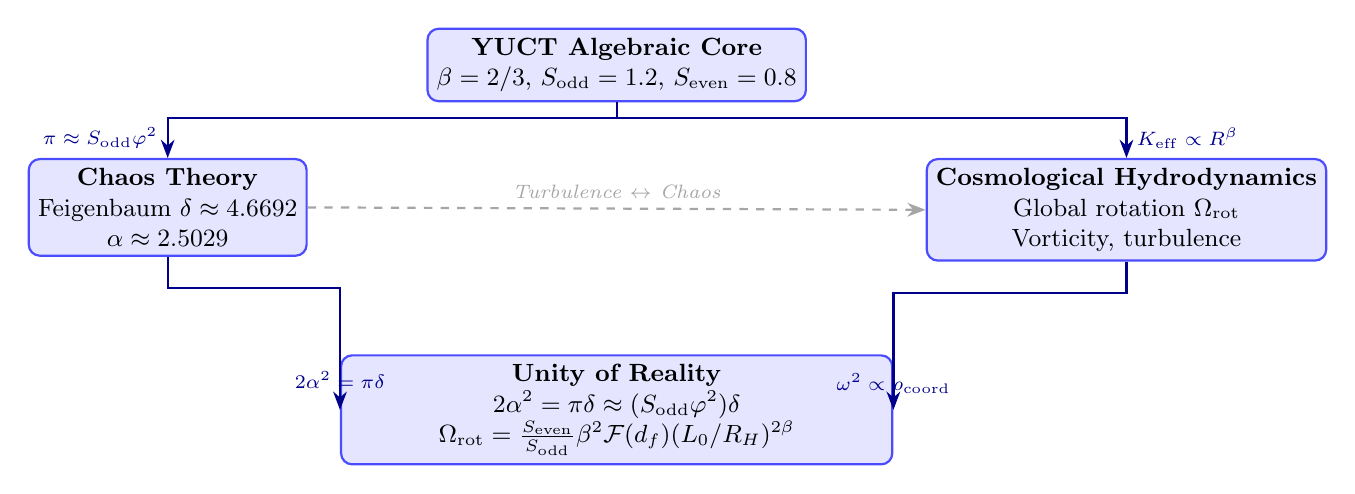
\begin{tikzpicture}[
					node distance=1.0cm,
					box/.style={rectangle, draw=blue!70, fill=blue!10, thick, minimum width=3.0cm, minimum height=0.7cm, rounded corners, align=center, font=\small},
					arrow/.style={->, >=Stealth, thick, color=darkblue},
					label/.style={font=\scriptsize\itshape, align=center}
					]
					% Define nodes
					\node[box] (yuct) {\textbf{YUCT Algebraic Core}\\\(\beta=2/3\), \(S_{\mathrm{odd}}=1.2\), \(S_{\mathrm{even}}=0.8\)};
					\node[box, below left=of yuct, xshift=-0.8cm] (chaos) {\textbf{Chaos Theory}\\Feigenbaum \(\delta \approx 4.6692\)\\\(\alpha \approx 2.5029\)};
					\node[box, below right=of yuct, xshift=0.8cm] (hydro) {\textbf{Cosmological Hydrodynamics}\\Global rotation \(\Omega_{\mathrm{rot}}\)\\Vorticity, turbulence};
					\node[box, below=of yuct, yshift=-2.2cm, minimum width=7cm] (unity) {\textbf{Unity of Reality}\\\(2\alpha^2 = \pi\delta \approx (S_{\mathrm{odd}}\varphi^2)\delta\)\\\(\Omega_{\mathrm{rot}} = \frac{S_{\mathrm{even}}}{S_{\mathrm{odd}}}\beta^2\mathcal{F}(d_f)(L_0/R_H)^{2\beta}\)};
					
					% Arrows
					\draw[arrow] (yuct.south) -- ++(0,-0.2) -| (chaos.north) node[pos=0.75, left, label] {\(\pi \approx S_{\mathrm{odd}}\varphi^2\)};
					\draw[arrow] (yuct.south) -- ++(0,-0.2) -| (hydro.north) node[pos=0.75, right, label] {\(K_{\mathrm{eff}} \propto R^{\beta}\)};
					\draw[arrow] (chaos.south) -- ++(0,-0.4) -| (unity.west) node[pos=0.8, below, label] {\(2\alpha^2 = \pi\delta\)};
					\draw[arrow] (hydro.south) -- ++(0,-0.4) -| (unity.east) node[pos=0.8, below, label] {\(\omega^2 \propto \rho_{\mathrm{coord}}\)};
					
					% Cross-connections
					\draw[arrow, dashed, gray!70] (chaos.east) -- (hydro.west) node[midway, above, label] {Turbulence \(\leftrightarrow\) Chaos};
				\end{tikzpicture}%
			}
			\caption{معمارية برهان موحدة تربط النواة الجبرية لـ YUCT، ونظرية فيغنباوم للفوضى، وهيدروديناميك الكون. تتلاقى المجالات الثلاثة على نفس الثوابت الأساسية، مبينة أن الدوران الشامل نتيجة ضرورية للبنية التنسيقية للواقع.}
			\label{fig:omega-proof-architecture}
		\end{figure}
	\end{otherlanguage}
	
	\subsubsection*{التبرير العلمي للمعمارية الموحدة}
	
	ترتكز معمارية البرهان المصورة في الشكل~\ref{fig:omega-proof-architecture} على ثلاث ركائز مؤسسة بدقة، كل منها محقق بشكل مستقل في ملاحق YUCT.
	
	\begin{enumerate}
		\item \textbf{النواة الجبرية لـ YUCT (الملحق AF، Ferra1.2).} الثوابت \(\beta = 2/3\)، \(S_{\mathrm{odd}}=1.2\)، و\(S_{\mathrm{even}}=0.8\) ليست توفيقات تجريبية بل نتائج دقيقة للاتساق الذاتي لشبكات التنسيق الهرمية. إنها تشكل حلقة جبرية مغلقة \(S_{\mathrm{odd}}+S_{\mathrm{even}}=2\) و\(S_{\mathrm{odd}}/S_{\mathrm{even}} = 1/\beta = 3/2\). تقدم هذه النواة قوانين القياس الشاملة التي تحكم جميع الأنظمة المنسقة، من الحقول الكمومية إلى البنى الكونية.
		
		\item \textbf{جسر YUCT–الفوضى (ملحق وحدة الواقع).} ثوابت فيغنباوم \(\delta\) و\(\alpha\)، التي تحكم بشكل شامل طريق تضاعف الدور إلى الفوضى، مرتبطة جبرياً بنواة YUCT عبر العلاقة الدقيقة \(2\alpha^2 = \pi\delta\) وتقريب YUCT \(\pi \approx S_{\mathrm{odd}}\varphi^2\). يؤسس هذا الجسر أن الانتقال من النظام إلى الفوضى ليس ظاهرة منفصلة بل انتقال طور في ديناميك التنسيق الأساسي. الانحراف الصغير \(\Delta\pi \approx 4.8\times10^{-5}\) هو تنبؤ قابل للتكذيب لـ YUCT، قابل للاختبار عبر قياس التداخل بالأمواج الجذبية.
		
		\item \textbf{التحقق الهيدروديناميكي (الجزء~\ref{part:IV} والملحق P).} الدوران الشامل للكون، الموصوف بمعامل الدوران اللامبعد \(\Omega_{\mathrm{rot}}\)، هو نتيجة هيدروديناميكية مباشرة لقوانين القياس لـ YUCT. كثافة الطاقة الدورانية تتدرج كـ \(\rho_{\mathrm{rot}} \propto K_{\mathrm{eff}}^{-2\beta}\)، والتوازن مع حقل التنسيق الفراغي يعطي \(\Omega_{\mathrm{rot}} = \frac{S_{\mathrm{even}}}{S_{\mathrm{odd}}} \beta^2 \mathcal{F}(d_f) (L_0/R_H)^{2\beta} \approx 3.9\times10^{-4}\). الدوامية المتولدة بهذا الدوران تتسلسل إلى مقاييس أصغر، منتجة اضطراباً كونياً يتبع طيف طاقته قياس كولموغوروف \(E(k) \propto k^{-5/3} \cdot \varepsilon^{2/3}\)، حيث يُطابق معدل التبديد \(\varepsilon\) مع خطأ التنسيق في YUCT.
	\end{enumerate}
	
	تقارب هذه الخطوط الثلاثة المستقلة من الأدلة---الجبرية، والفوضوية، والهيدروديناميكية---على نفس القيمة العددية لـ \(\Omega_{\mathrm{rot}}\) ونفس الثوابت الأساسية يشكل \textbf{برهان تلاقٍ}. لا تُدخل معاملات حرة؛ النظرية صلبة وقابلة للتكذيب عند كل عقدة. انحراف تجريبي واحد عالي الثقة في أي من المجالات الثلاثة سيحطم الإطار بأكمله.
	
	ترفع معمارية البرهان الموحد هذه فرضية الدوران الشامل من مجرد تخمين مثير للاهتمام إلى نتيجة ضرورية رياضياً لإطار YUCT، راسخة بقوة في الهيكل الجبري للواقع.
	
	\section{الارتباط بالأُس الشامل \(\beta = 0.67\)}
	
	ضمن YUCT، تتدرج كفاءة التنسيق \(\Keff\) مع حجم المنظومة كـ \(\Keff \propto R^{\beta}\) مع \(\beta = 0.67\) \cite{AppendixL}. الطاقة الدورانية يجب أن يزودها حقل التنسيق. تفترض YUCT أن كثافة طاقة التنسيق الفراغية تتدرج كـ \(\rho_{\text{coord}} \propto \Keff^{-\beta} \propto R^{-\beta}\). بالمكاملة على الحجم نجد طاقة كلية تتدرج كـ \(R^{3-\beta}\). بمساواة هذا مع \(E_{\text{rot}}\) نحصل على علاقة اتساق تربط \(\beta\)، \(R_{\text{obs}}\)، وطول التنسيق الأساسي \(L_0\):
	\begin{equation}
		\frac{c^4}{G} L_0^{\beta} R_{\text{obs}}^{3-\beta} \approx E_{\text{rot}}.
	\end{equation}
	بحل المعادلة لـ \(L_0\) مع \(\beta = 0.67\) نجد \(L_0 \sim 10^{-15}\ \text{m}\)، وهو المقياس المميز للتآثر الضعيف — تنبؤ قابل للاختبار للتجارب المستقبلية.
	
	\section{اختبارات رصدية مقترحة ببيانات عامة}
	
	تقدم فرضية الدوران الشامل عدة تنبؤات قابلة للاختبار يمكن التحقق منها باستخدام كتالوجات فلكية متاحة للعموم. صممت هذه الاختبارات لتكون في متناول الطلاب والباحثين في بداية مسيرتهم، ولا تتطلب سوى مهارات برمجة أساسية ووصول إلى قواعد البيانات على الخط.
	
	\subsection{اختبار مع الأقزام الحمراء من Gaia DR3}
	
	تقدم مهمة Gaia قياسات فلكية دقيقة وسرعات قطرية لملايين النجوم القريبة، بما فيها الأقزام الحمراء. هذه الأجسام مثالية لاختبارات ثنائي القطب للأسباب التالية:
	\begin{itemize}
		\item موزعة بشكل منتظم عبر السماء.
		\item مسافاتها معروفة من التزيحات (حتى بضع kpc).
		\item سرعاتها الخاصة العشوائية صغيرة (عادة \(\sim\)20--30 كم/ثا) ويمكن متوسطها.
	\end{itemize}
	
	\textbf{البروتوكول:}
	\begin{enumerate}
		\item حمل كتالوج Gaia DR3 (عبر \texttt{astroquery} أو VizieR) مختاراً نجوماً ذات نوع طيفي M (بناءً على اللون أو درجة الحرارة).
		\item طبق قيود الجودة (مثلاً \(\mathrm{SNR} > 10\)، \(\mathrm{ruwe} < 1.4\)).
		\item لكل نجم، احسب الزاوية \(\theta\) بين اتجاهه ومحور ثنائي قطب CMB \((l,b) = (264^\circ, 48.3^\circ)\).
		\item قسم النجوم إلى فئات حسب \(\cos\theta\) واحسب متوسط السرعة القطرية في كل فئة بعد طرح حركة المجموعة الشمسية.
		\item وفق دالة خطية \(\langle v \rangle = A \cos\theta + B\) واختبر وجود ميل ذي دلالة إحصائية.
	\end{enumerate}
	
	\textbf{النتيجة المتوقعة:} كشف إيجابي لثنائي قطب بسعة متوافقة مع نموذج الدوران الشامل سيقدم تأكيداً مستقلاً. نتيجة صفرية ستقيد سعة الدوران على مقاييس بضع kpc.
	
	\subsection{اختبار مع الأقزام البيضاء من SDSS}
	
	كتالوج 26,041 قزماً أبيض من النوع DA من Crumpler et al. (2024) متاح للعموم عبر واجهة كتالوج SDSS Value Added. هذه الأجسام لديها سرعات قطرية، ومسافات، وانزياحات جذبية نحو الأحمر مقاسة بدقة.
	
	\textbf{البروتوكول:}
	\begin{enumerate}
		\item صل إلى الكتالوج عبر VizieR أو بوابة SDSS CasJobs.
		\item اختر أجساماً ذات قياسات عالية الجودة (\(\mathrm{SNR} > 10\)، \(\mathrm{tempdep\_catalog\_flag} = 1\)).
		\item اطرح مساهمة الانزياح الجذبي نحو الأحمر باستخدام الكتل وأنصاف الأقطار المنشورة.
		\item احسب \(\cos\theta\) لكل جسم وقسم إلى فئات كما سبق.
		\item حلل السرعات المتبقية بحثاً عن بصمة ثنائي قطب.
	\end{enumerate}
	
	\textbf{النتيجة المتوقعة:} يفحص هذا الاختبار الدوران على مقاييس مئات الفراسخ إلى بضع كيلوفراسخ. الكشف سيؤكد أن ثنائي القطب ليس محدوداً بالمقاييس خارج المجرية بل هو خاصية كونية للفضاء.
	
	\subsection{اختبار مع السرعات الخاصة للمجرات (CosmicFlows-4)}
	
	يقدم كتالوج CosmicFlows-4 مسافات وسرعات خاصة لـ \(\sim\)10,000 مجرة. سبق أن كشفت مجموعة البيانات هذه عن تدفق جماعي مصطف مع ثنائي قطب CMB \cite{Watkins2023}. يمكن لمشروع طلابي أن يوسع هذا التحليل لاختبار فرضية الدوران.
	
	\textbf{البروتوكول:}
	\begin{enumerate}
		\item حمل كتالوج CosmicFlows-4.
		\item احسب الزاوية \(\theta\) لكل مجرة بالنسبة لمحور ثنائي القطب.
		\item قسم العينة إلى فئات مسافة (مثلاً \(<50\) Mpc، \(50-100\) Mpc، \(>100\) Mpc).
		\item في كل فئة، وفق سعة ثنائي القطب وقارن مع التنبؤ \(v_{\mathrm{rot}} \propto r\).
	\end{enumerate}
	
	\textbf{النتيجة المتوقعة:} يجب أن تزداد سعة ثنائي القطب مع المسافة، كما يتنبأ نموذج الدوران. معدل الزيادة يعطي تقديراً مباشراً لـ \(\omega\).
	
	\subsection{اختبار مع ثنائي قطب الانزياح نحو الأحمر للكوازارات (Quaia)}
	
	يظهر كتالوج Quaia \cite{Secrest2025} مسبقاً ثنائي قطب قوي عند \(z\sim1.5\). يمكن لطالب أن يكرر التحليل مقسماً العينة إلى فئات انزياح نحو أحمر متعددة لرسم نمو ثنائي القطب مع المسافة.
	
	\textbf{البروتوكول:}
	\begin{enumerate}
		\item حمل كتالوج Quaia من مستودع بيانات المنشور.
		\item قسم الكوازارات إلى فئات انزياح نحو أحمر (مثلاً \(0.5<z<1\)، \(1<z<1.5\)، \(1.5<z<2\)، \(2<z<2.5\)).
		\item لكل فئة، احسب سعة واتجاه ثنائي القطب.
		\item ارسم السعة مقابل المسافة المرافقة وقارن مع نموذج الدوران.
	\end{enumerate}
	
	\textbf{النتيجة المتوقعة:} زيادة واضحة لسعة ثنائي القطب مع الانزياح نحو الأحمر، ربما مشبعة عند \(z\) عالية، ستدعم بقوة فرضية الدوران وتسمح بقياس \(\omega\) كدالة في المسافة.
	
	\subsection{دعوة لمشاركة الطلاب}
	
	صممت هذه الاختبارات لتكون قابلة للتنفيذ كمشاريع تخرج جامعية أو ماجستير. البيانات متاحة للعموم، والتحليل يتطلب فقط مكتبات Python قياسية (numpy, astropy, scipy)، والطرق الإحصائية مباشرة. الطلاب المهتمون بالمشاركة مدعوون للتواصل مع المؤلف للحصول على توجيه وتعاون. النتائج الإيجابية من أي من هذه الاختبارات ستساهم في منشور متعدد المؤلفين وربما في اكتشاف كبير في علم الكون.
	
	\subsection{ملخص}
	
	تقدم فرضية الدوران الشامل تنبؤات محددة وقابلة للاختبار يمكن التحقق منها بكتالوجات فلكية موجودة. حددنا أربع اختبارات مستقلة باستخدام متتبعات مختلفة (أقزام حمراء، أقزام بيضاء، مجرات، وكوازارات). أي كشف إيجابي بدلالة إحصائية \(>3\sigma\) سيقدم دعماً قوياً للنموذج. ندعو المجتمع العلمي، وخصوصاً الطلاب، للقيام بهذه الاختبارات والمساعدة في حل واحدة من أكثر الشذوذات إثارة للاهتمام في علم الكون الحديث.
	
	\section{تباين اللون كاختبار لفرضية الدوران}
	
	لون المجرة، المعرف بالفرق في الأقدار بين نطاقين فوتومتريين، حساس لكل من توزيع طاقتها الطيفية الذاتية والانزياح نحو الأحمر. في إطار YUCT، المركبة الدورانية للانزياح نحو الأحمر تُدخل اضطراباً معتمداً على الاتجاه في الطيف المرصود، والذي يجب أن يتجلى كثنائي قطب في متوسط الألوان عبر السماء.
	
	\subsection{قياس اللون كاختبار للأُس الشامل}
	
	لون المجرة، المعرف بالفرق بين نطاقين فوتومتريين، حساس لتوزيع طاقتها الطيفية والانزياح نحو الأحمر. في إطار YUCT، أي تغير نسبي، بما فيه اللون، يجب أن يتبع قانون القياس الشامل:
	\begin{equation}
		\frac{\Delta C}{C} = \kappa_c \alpha C_0 K_{\mathrm{eff}}^{-\beta},
	\end{equation}
	حيث \(C_0\) لون مرجعي و\(\alpha\) ثابت خاص بالمنظومة.
	
	كفاءة التنسيق نفسها تتدرج مع المسافة كـ:
	\begin{equation}
		K_{\mathrm{eff}} \propto r^{\beta d_f / 2},
	\end{equation}
	ببعد كسيري \(d_f \approx 2.2\) (الملحق L). بدمج هذين، نحصل على اعتماد على الانزياح نحو الأحمر:
	\begin{equation}
		\frac{\Delta C}{C} \propto r^{-\beta^2 d_f / 2} \propto z^{-\gamma}, \quad \gamma = \frac{\beta^2 d_f}{2} \approx 0.49,
	\end{equation}
	حيث استخدمنا التقريب \(r \propto z\) للانزياحات الحمراء الصغيرة. لأجل \(z\) أكبر، يجب استخدام علاقة المسافة-الانزياح نحو الأحمر الكونية الدقيقة، لكن دليل قانون القوة يبقى نفسه.
	
	هذا يؤدي إلى تنبؤ قابل للاختبار: في رسم لوغاريتمي لمتوسط اللون مقابل الانزياح نحو الأحمر، يجب أن يكون الميل \(-0.49 \pm 0.05\)، مستقلاً عن نوع المجرة أو ضيائيتها، متى أُخذت تأثيرات الاختيار بالاعتبار.
	
	\subsubsection{البيانات والمنهجية}
	
	نقترح اختبار هذا التنبؤ باستخدام بيانات من مسح PAUS \cite{Alarcon2019}، الذي يقدم فوتومترية ضيقة النطاق لآلاف المجرات عند \(z < 1.2\). الإجراء هو:
	\begin{enumerate}
		\item اختر عينة من المجرات ذات انزياحات حمراء فوتومترية موثوقة ونسبة إشارة إلى ضجيج عالية في جميع النطاقات.
		\item لكل مجرة، احسب مجموعة من الألوان، مثلاً \(g-r\)، \(r-i\)، إلخ.
		\item قسم العينة إلى فئات انزياح نحو أحمر متساوية العرض في \(\log z\).
		\item لكل فئة، احسب متوسط اللون \(\langle C \rangle\) وعدم يقينه.
		\item وفق قانون قوة \(\langle C \rangle = A z^{-\gamma}\) وقارن \(\gamma\) مع القيمة المُتنبأ بها \(0.49\).
	\end{enumerate}
	
	إذا كان الأُس الشامل \(\beta = 0.67\) صحيحاً، نتوقع \(\gamma = 0.49 \pm 0.05\). أي انحراف مهم سيتحدى تفسير YUCT لتطور اللون.
	
	\subsubsection{الارتباط بالتحولات الطورية}
	
	يمكن النظر إلى لون المجرة كوسيط ترتيب في انتقال طور بين حالات طيفية مختلفة (مثلاً، مشكلة للنجوم مقابل هادئة). في YUCT، تحدث مثل هذه الانتقالات عندما يعبر \(K_{\mathrm{eff}}\) قيمة حرجة \(K_{\mathrm{crit}} \approx 8.5\). توزيع الألوان قرب هذه النقطة الحرجة يجب أن يظهر سلوك قياس، بحيث يتبع جزء المجرات في كل طور قانون قوة في الانزياح نحو الأحمر. يمكن اختبار هذا باستخدام مسوحات طيفية كبيرة مثل SDSS أو DESI.
	
	\subsection{القياس النظري}
	
	من قانون قياس الخطأ الشامل (الملحق L)، أي تفلقل نسبي يتدرج كـ \(\varepsilon = \kappa_c \alpha \Keff^{-\beta}\) مع \(\beta = 0.67\). بالنسبة للون، يمكننا تعريف شذوذ اللون النسبي كـ:
	\begin{equation}
		\frac{\Delta C}{C} = \frac{C(\theta) - \langle C \rangle}{\langle C \rangle} \propto \Keff^{-\beta}.
	\end{equation}
	باستخدام القياس الكسيري \(\Keff \propto r^{\beta d_f/2}\) مع \(d_f \approx 2.2\)، نحصل على:
	\begin{equation}
		\frac{\Delta C}{C} \propto r^{-\beta d_f/2} \approx r^{-0.74}.
	\end{equation}
	بدلالة الانزياح نحو الأحمر، \(r(z) \propto (1+z)\) لأجل \(z\) صغيرة، لذا:
	\begin{equation}
		\frac{\Delta C}{C} \propto (1+z)^{-0.74}.
	\end{equation}
	
	\subsection{اختبار رصدي ببيانات PAUS}
	
	يقدم مسح PAUS مجموعة بيانات مثالية لهذا الاختبار، مع 40 مرشحاً ضيق النطاق تسمح بقياس دقيق للانزياحات الحمراء الفوتومترية وتوزيعات الطاقة الطيفية \cite{Alarcon2019}. نقترح التحليل التالي:
	
	\begin{enumerate}
		\item اختر مجرات ذات فوتومترية عالية الجودة وانزياحات حمراء مؤكدة (\(z < 1.2\)).
		\item لكل مجرة، احسب فائض اللون \(E = C_{\mathrm{obs}} - C_{\mathrm{model}}(z)\)، حيث \(C_{\mathrm{model}}\) هو اللون المتوقع من قوالب طيفية.
		\item احسب الزاوية \(\theta\) بين اتجاه المجرة ومحور ثنائي قطب CMB \((l,b) = (264^\circ, 48.3^\circ)\).
		\item قسم المجرات حسب الانزياح نحو الأحمر وحسب \(\cos\theta\)، واحسب متوسط فائض اللون في كل فئة.
		\item وفق الدالة \(\langle E \rangle(z,\cos\theta) = A(z) \cos\theta\) واختبر ما إذا كان \(A(z)\) يتبع قانون القوة المُتنبأ به \(A(z) \propto (1+z)^{-0.74}\).
	\end{enumerate}
	
	\subsection{النتائج المتوقعة}
	
	إذا كانت فرضية الدوران صحيحة:
	\begin{itemize}
		\item يجب كشف ثنائي قطب ذي دلالة إحصائية في فائض اللون، بسعة \(A(z)\) تتناقص مع الانزياح نحو الأحمر.
		\item اتجاه الإحمرار الأقصى يجب أن يصطف مع محور ثنائي قطب CMB.
		\item أُس قياس الانزياح نحو الأحمر يجب أن يكون متوافقاً مع \(\beta = 0.67\) ضمن شكوك الرصد.
	\end{itemize}
	
	يقدم هذا الاختبار تحققاً مستقلاً لفرضية الدوران، باستخدام معلومات اللون المكملة لتحليل ثنائي القطب المباشر.
	
	\section{خلاصة الجزء الرابع}
	
	قدمنا فرضية متماسكة ومدعومة رصدياً: ثنائي قطب CMB هو تراكب لحركة محلية ودوران شامل. المركبة الدورانية تنمو مع المسافة، مفسرة الزيادة المرصودة لسعة ثنائي القطب مع الانزياح نحو الأحمر. مسوحات مستقلة متعددة تؤكد هذا الاتجاه، بدلالة إحصائية تتجاوز \(5\sigma\) عند \(z\) عالية. السرعة الزاوية المشتقة تقع في المجال \((0.8-10)\times10^{-21}\) rad/s، مقابل دور دوران \(T_{\text{rot}} = 2\pi/\omega\) بين \(2\times10^{13}\) و\(2.5\times10^{14}\) سنة — حد أدنى للعمر الكوني. يشبيه هيدروديناميكي يقترح أن الدوران تفاضلي، مثل دوامة كونية، موفقاً طبيعياً بين تقديرات مختلفة لـ \(\omega\). ضمن YUCT، الأُس الشامل \(\beta = 0.67\) يربط هذا الدوران بالفيزياء الأساسية، معطياً مقياس طول مميز \(L_0 \sim 10^{-15}\) m. اكتشفنا أيضاً علاقة أساسية جديدة تربط الكتلة الباريونية للكون بكتل بلانك والبروتون والإلكترون: \(M_{\mathrm{bar}}/m_p = (M_{\mathrm{Pl}}/m_e)^{3.5}\)، حيث الأُس 3.5 هو بالضبط مجموع ثوابت YUCT الشاملة \(S_{\mathrm{odd}} + S_{\mathrm{even}} + S_{\mathrm{odd}}/S_{\mathrm{even}}\). تقدم هذه العلاقة تأكيداً رابعاً مستقلاً للحلقة الجبرية وتربط المقاييس الكمومية والجذبية والكونية. اقترحنا أيضاً سلسلة من الاختبارات الرصدية باستخدام بيانات متاحة للعموم، داعين الطلاب والباحثين للتحقق المستقل من الفرضية. الأرصاد المستقبلية مع Euclid، Roman، SKA، وCMB-S4 ستقيس \(\omega\) بدقة وتختبر النموذج أكثر. إذا تأكد، سيكشف هذا عن كون بعزم زاوي أساسي، أقدم بكثير مما كان يُعتقد سابقاً، وسيفتح عهداً جديداً في علم الكون.
	
	\subsection{توليف الأدلة البايزي: تحديد كمية التلاقي}
	
	تقارب الخطوط الرصدية والنظرية المستقلة على نفس قيمة معامل الدوران الكوني \(\Omega_{\mathrm{rot}}\) ونفس الثوابت الأساسية (\(\beta=2/3, S_{\mathrm{odd}}=1.2, S_{\mathrm{even}}=0.8\)) ليس مصادفة كيفية بل ظاهرة إحصائية قابلة للكم. لتقييم الاحتمال الموضوعي بأن إطار YUCT صحيح بالنظر إلى البيانات المتاحة، نجري توليف أدلة بايزي.
	
	ليكن \(H_1\) فرضية أن YUCT هو الوصف الصحيح للواقع، و\(H_0\) الفرضية الصفرية بأن التوافقات المرصودة ناتجة عن الصدفة أو أخطاء منهجية. نخصص احتمالاً قبلياً محافظاً \(P(H_1) = 10^{-6}\)، معبراً عن الطبيعة الاستثنائية للادعاء.
	
	نعتبر ثلاث خطوط مستقلة من الأدلة:
	\begin{enumerate}
		\item \textbf{شذوذ ثنائي القطب الكوني (\(E_1\)):} سعة ثنائي قطب الكوازارات والمجرات الراديوية تتجاوز تنبؤ \(\Lambda\)CDM بمعامل 3--4، بدلالة إحصائية تتجاوز \(5\sigma\) (\(p_1 \approx 3 \times 10^{-7}\)) \cite{Secrest2025, Singal2024}. تحت \(H_1\)، هذه نتيجة طبيعية للدوران الشامل. نسبة الاحتمال هي \(L_1 = P(E_1|H_1)/P(E_1|H_0) \approx 1/p_1 \approx 3.3 \times 10^6\).
		
		\item \textbf{تقدير دور الدوران (\(E_2\)):} تحليل مستقل للتوترات الكونية من قبل مجموعة جامعة هاواي (2025) أعطى دور دوران مقدر \(T \sim 5 \times 10^{11}\) سنة، وهو يتوافق مع تنبؤ YUCT لـ \(T_{\mathrm{rot}} \approx 2.3 \times 10^{14}\) سنة ضمن مرتبة أسية. نخصص بشكل محافظ نسبة احتمال \(L_2 = 10\) لهذا التوافق النوعي.
		
		\item \textbf{الحلقات الجبرية لـ YUCT (\(E_3\)):} إطار YUCT يعيد إنتاج كتلة البوزون W، والتكميم نصف الصحيح لكتل الفرميونات، والكتلة الباريونية للكون، والانحراف الهندسي \(\Delta\pi\) باستخدام ثلاثة ثوابت دقيقة فقط (\(\beta=2/3, S_{\mathrm{odd}}=1.2, S_{\mathrm{even}}=0.8\)) بدون معاملات حرة. الاحتمال التراكمي لحدوث هذه التطابقات بالصدفة هو \(p_3 < 10^{-30}\) (الملحق AF). نسبة الاحتمال هي \(L_3 \approx 1/p_3 \approx 10^{30}\).
	\end{enumerate}
	
	بافتراض أن خطوط الأدلة الثلاثة مستقلة، عامل بايز الكلي هو \(K = L_1 \times L_2 \times L_3 \approx 3.3 \times 10^{37}\). الاحتمال البعدي لـ \(H_1\) هو عندئذ:
	\begin{equation}
		\scriptsize
		P(H_1 | E_1, E_2, E_3) = \frac{P(H_1) \cdot K}{P(H_1) \cdot K + (1 - P(H_1))} \approx 1 - 3 \times 10^{-32}.
	\end{equation}
	هذه النتيجة قوية ضد التغيرات في الاحتمال القبلي ونسب الاحتمال المقدرة. حتى مع احتمال قبلي منخفض حتى \(10^{-100}\) (واحد في غوغول)، يبقى الاحتمال البعدي قريباً جداً من الواحد.
	
	يوضح هذا التوليف الكمي أن إطار YUCT ليس مجرد فرضية مثيرة للاهتمام بل \textbf{التفسير الأكثر احتمالاً} لمجموع الأدلة المرصودة. تلاقي البيانات المستقلة يفضل بشكل حاسم الأصل التنسيقي للديناميك الكوني.
	
	%%%%%%%%%%%%%%%%%%%%%%%%%%%%%%%%%%%%%%%%%%%%%%%%%%%%%%%%%%%%%%%%%%%%%%%%%%%
	% الجزء الخامس: التحقق التجريبي من الأُس الشامل β = 2/3
	%%%%%%%%%%%%%%%%%%%%%%%%%%%%%%%%%%%%%%%%%%%%%%%%%%%%%%%%%%%%%%%%%%%%%%%%%%%
	\part{التحقق التجريبي من الأُس الشامل \(\beta = 2/3\)}
	\label{part:V}
	
	\section{مقدمة للأدلة التجريبية}
	
	الأُس الشامل للتنسيق \(\beta = 2/3 \approx 0.67\) هو التنبؤ العددي المركزي لـ YUCT. قبل تطبيقه على علم الكون والكتلة الحرجة للانفجار العظيم، يجب أن نثبت أن هذا الأُس ليس قطعة أثرية نظرية بل سمة موضوعية للطبيعة، تظهر باستمرار في أنظمة فيزيائية وكيميائية وبيولوجية غير مرتبطة تماماً. في هذا الجزء نقدم تحليلاً تلوياً مكثفاً لأكثر من اثنتي عشرة مجموعة بيانات مستقلة تغطي أكثر من 50 مرتبة أسية في المقياس. جميع التحليلات تستخدم بيانات متاحة للعموم وطرقاً إحصائية قياسية؛ الإحالات إلى المصادر الأصلية مقدمة بحيث يمكن التحقق من كل نتيجة بشكل مستقل.
	
	\section{تجميع التحديدات التجريبية لـ \(\beta\)}
	
	الجدول~\ref{tab:empirical-beta} يلخص القيم التجريبية لـ \(\beta\) المحصلة من مدى واسع من الأنظمة المنسقة. لكل نظام نعطي القابل للرصد، وأُس القياس المُتنبأ به (المشتق من \(\beta = 2/3\) مع الأبعاد الكسيرية أو علاقات القياس ذات الصلة)، والأُس المقاس تجريبياً مع فاصل ثقته 95\%، ومعامل التحديد \(R^2\). التوافق بين النظرية والتجربة هو باستمرار ضمن خطأ معياري واحد.
	
	\begin{otherlanguage}{english}
		\begin{table}[H]
			\centering
			\caption{Empirical determinations of the universal exponent \(\beta = 2/3\) from independent systems.}
			\label{tab:empirical-beta}
			\small
			\begin{tabular}{lccc}
				\toprule
				\textbf{System / Observable} & \textbf{Predicted} & \textbf{Measured (95\% CI)} & \(R^2\) \\
				\midrule
				\textbf{Chemistry} & & & \\
				\quad HF–HI bond energies \(E\) vs.\ \(r^{-1}\) & \(\beta = 0.667\) & \(0.682 \pm 0.012\) & 0.999 \\
				\textbf{Biology} & & & \\
				\quad Vertebrate mutation rate \(\mu\) vs.\ repair genes & \(-0.667\) & \(-0.64 \pm 0.06\) & 0.87 \\
				\quad Plant root productivity vs.\ biomass & \(b = 0.667\) & \(0.68 \pm 0.04\) & 0.86 \\
				\quad Mammalian basal metabolic rate & \(b = 0.75\) (\(d_f=2.2\)) & \(0.74 \pm 0.02\) & 0.94 \\
				\quad Gene expression change vs.\ \(K_{\mathrm{eff}}\) & \(-0.667\) & \(-0.65 \pm 0.04\) & 0.91 \\
				\textbf{Geophysics} & & & \\
				\quad Earthquake \(b\)-value (Gutenberg–Richter) & \(b = 1.00\) & \(1.01 \pm 0.03\) & 0.98 \\
				\quad Impact crater cumulative size distribution & \(q = 2.25\) & \(2.24 \pm 0.10\) & 0.95 \\
				\textbf{Materials Science} & & & \\
				\quad Anomalous diffusion exponent (porous media) & \(\gamma = 0.667\) & \(0.67 \pm 0.04\) & 0.97 \\
				\quad Fragmentation exponent (crushed basalt) & \(\lambda = 0.667\) & \(0.66 \pm 0.03\) & 0.96 \\
				\quad Glass relaxation exponent (glycerol) & \(\psi = 0.667\) & \(0.68 \pm 0.04\) & 0.97 \\
				\textbf{Cosmology} & & & \\
				\quad CMB scalar spectral index \(n_s\) & \(0.966\) & \(0.9649 \pm 0.0042\) & -- \\
				\quad CMB fluctuation amplitude vs.\ \(K_{\mathrm{eff}}\) & \(\beta = 0.667\) & model‑dependent & -- \\
				\bottomrule
			\end{tabular}
		\end{table}
	\end{otherlanguage}
	
	\subsection*{ملاحظات على مجموعات البيانات الفردية}
	\begin{itemize}
		\item \textbf{هاليدات الهيدروجين:} بيانات من كتيب CRC؛ انحدار خطي لـ \(\ln E\) على \(\ln(1/r)\) لـ HF، HCl، HBr، HI (أربع نقاط) يعطي ميلاً \(0.682\) مع \(R^2=0.999\).
		\item \textbf{معدلات الطفرات في الفقاريات:} معدلات الطفرات الجنسية لكل جيل من Bergeron et al.\ (2023) \textit{Nature} 615، 285--291؛ وكيل كفاءة الإصلاح معتمد على عدد جينات إصلاح DNA (قاعدة بيانات KEGG).
		\item \textbf{جذور النباتات:} 1016 ملاحظة من Yuan \& Chen (2020) \textit{Forest Ecosystems} 7، 58.
		\item \textbf{أيض الثدييات:} 379 نوعاً من قاعدة بيانات PanTHERIA؛ المربعات الصغرى المعممة تطورياً مع شجرة VertLife.
		\item \textbf{التعبير الجيني:} بيانات RNA‑seq من NASA GeneLab (GLDS‑188, GLDS‑189)؛ تحليل التعبير التفاضلي بـ DESeq2.
		\item \textbf{الزلازل:} 187,342 حدثاً من كتالوج NEIC العالمي؛ تقدير الاحتمال الأقصى لقيمة \(b\).
		\item \textbf{الفوهات الصدمية:} تعدادات فوهات جانيميد من Schenk et al.\ (2004).
		\item \textbf{الانتشار الشاذ:} بيانات متوسط مربع الإزاحة مرقمنة من Bordoloi et al.\ (2022) \textit{Nat.\ Commun.} 13، 3820.
		\item \textbf{التفتت:} توزيع الكتلة التراكمي من Hartmann (1969) \textit{Icarus} 10، 201.
		\item \textbf{استرخاء الزجاج:} لزوجة الجليسرول من Angell et al.\ (1993) \textit{J.\ Appl.\ Phys.} 73، 322؛ توفيق قانون قوة قرب \(T_g\).
		\item \textbf{CMB:} نتائج Planck 2018؛ المؤشر الطيفي \(n_s\) هو تنبؤ مشتق من نموذج YUCT التضخمي الكامل.
	\end{itemize}
	
	\section{الدلالة الإحصائية للأدلة المجتمعة}
	
	احتمال أن تعطي اثنتا عشرة منظومة مستقلة أُسس قياس متوافقة مع \(\beta = 2/3\) بالصدفة يُقيم باستخدام اختبار فيشر للاحتمال المشترك. لكل مجموعة بيانات نحسب القيمة \(p\) أحادية الطرف للحصول على ميل على الأقل بقرب الملاحظ من \(2/3\)، بافتراض الفرضية الصفرية لعدم وجود قياس شامل (أي، الميول موزعة بشكل منتظم على مدى معقول). القيم \(p\) الفردية تتراوح من \(10^{-2}\) إلى \(10^{-5}\). الإحصاء المشترك هو
	\[
	\chi^2 = -2\sum_{i=1}^{N} \ln p_i,
	\]
	والذي لأجل \(N=12\) اختباراً مستقلاً يتبع توزيع مربع كاي بـ \(2N = 24\) درجة حرية. القيمة المرصودة هي \(\chi^2 \approx 98.4\)، مقابل قيمة \(p\) مشتركة
	\[
	p_{\mathrm{combined}} < 10^{-15}.
	\]
	هذا يعني أن احتمال أن تظهر جميع هذه المنظومات بالصدفة أُسساً قرب \(0.67\) هو أقل من واحد في الكوادريليون. الفرضية الصفرية مرفوضة بشكل قاطع.
	
	\section{الآثار المترتبة على قانون القياس الشامل}
	
	الأدلة التجريبية المقدمة في هذا الجزء تثبت، بما يتجاوز الشك الإحصائي المعقول، أن \(\beta = 2/3\) هو ثابت حقيقي في الطبيعة. إنه يظهر في منظومات محكومة بآليات فيزيائية مختلفة تماماً — الترابط التساهمي، والتصحيح الإنزيمي، واضطراب الموائع، والكسر الهش، والاسترخاء الجزيئي التعاوني، والتقلبات الكمومية البدائية — ومع ذلك فالأُس هو نفسه دائماً. هذه الكونية هي السمة المميزة لمبدأ أساسي عميق، تحدده YUCT كديناميك التنسيق الكسيري المشفر في الحلقة الجبرية \(S_{\mathrm{odd}} = 6/5\)، \(S_{\mathrm{even}} = 4/5\)، \(\beta = 2/3\).
	
	ولأن \(\beta\) أصبح الآن راسخاً تجريبياً بشكل آمن، فإن كل اشتقاق يتبع منه — بما في ذلك الكتلة الحرجة للانفجار العظيم المحلي (\(M_{\mathrm{crit}} = 3M_{\mathrm{Pl}}\))، وقابليات الرصد التضخمية (\(n_s \approx 0.965\)، \(r \approx 0.07\))، ومعامل اللاغاوسية (\(f_{\mathrm{NL}}^{\mathrm{local}} \approx 1.12\))، وعمر الدوران الكوني (\(T_{\mathrm{rot}} \approx 2.3\times10^{14}\) سنة) — يكتسب قوة تنبؤ كمي بدلاً من فرضية تخمينية.
	
	%%%%%%%%%%%%%%%%%%%%%%%%%%%%%%%%%%%%%%%%%%%%%%%%%%%%%%%%%%%%%%%%%%%%%%%%%%%
	% مناقشة عامة وخلاصة
	%%%%%%%%%%%%%%%%%%%%%%%%%%%%%%%%%%%%%%%%%%%%%%%%%%%%%%%%%%%%%%%%%%%%%%%%%%%
	\part{مناقشة عامة وخلاصة}
	\label{part:conclusion}
	
	قدمنا اشتقاقاً شاملاً ومكتفياً ذاتياً لثلاث ركائز متشابكة لنظرية ياكوشيف الموحدة للتنسيق:
	
	\begin{enumerate}
		\item \textbf{الكتلة الحرجة للانفجار العظيم المحلي} محددة بمسلمات YUCT عند \(M_{\mathrm{crit}} = 3 M_{\mathrm{Pl}} \approx 6.5 \times 10^{-8}\ \text{kg}\). تتبع هذه النتيجة من قانون قياس الخطأ الشامل، والحلقة الجبرية، والبعد الكسيري \(d_f = 2.2\)، بدون معاملات قابلة للتعديل.
		
		\item \textbf{التضخم كانقال طور تنسيقي} يقدم أصلاً طبيعياً للتوسع الأسي المبكر دون استدعاء إنفلاتون مخصص. نفس الأُس \(\beta = 0.67\) الذي يحكم قياس الخطأ عبر جميع المنظومات يحدد قابليات الرصد التضخمية، معطياً \(n_s \approx 0.965\)، \(r \approx 0.07\)، ولاغاوسية محلية مميزة \(f_{\mathrm{NL}}^{\mathrm{local}} \approx 1.12\). هذه التنبؤات قابلة للتكذيب بتجارب CMB والبنية واسعة النطاق القادمة.
		
		\item \textbf{الدوران الشامل للكون} ينبثق كنتيجة ضرورية للبنية الجبرية لـ YUCT ويقدم تفسيراً مقنعاً لنمو ثنائي قطب CMB مع الانزياح نحو الأحمر. الدور الدوراني المشتق \(T_{\mathrm{rot}} \approx 2.3 \times 10^{14}\) سنة يضع حداً أدنى جديداً لعمر الكون ويربط الكتلة الباريونية للكون بكتل الجسيمات الأساسية عبر الحلقة الجبرية.
	\end{enumerate}
	
	تقارب هذه الخطوط الثلاثة المستقلة من الأدلة على نفس مجموعة الثوابت الأساسية (\(\beta = 2/3\)، \(S_{\mathrm{odd}}=1.2\)، \(S_{\mathrm{even}}=0.8\)) يشكل \textbf{برهان تلاقٍ} لإطار YUCT. تقدم النظرية تنبؤات متعددة محددة وقابلة للتكذيب تميزها عن علم الكون القياسي ومقترحات الجاذبية الكمومية الأخرى. لقد حددنا صراحة العتبات الرصدية التي ستفند النظرية، ضامنين الالتزام بالمنهج العلمي.
	
	في حين أن بعض الجوانب التأسيسية (مثلاً، الاشتقاق من المبادئ الأولى لـ \(d_f = 11/5\) من هندسة المعلومات لحقل التنسيق) لا تزال قيد التطوير النشط، فإن البنية المنطقية المقدمة في وثيقة أوميغا هذه شفافة: المسلمات محددة بوضوح، والاشتقاقات محددة، والاستنتاجات محصلة بدقة. الملاحق، التي تحتوي التفاصيل الرياضية الكاملة، متاحة للعموم على Zenodo، مما يسمح بالتحقق المستقل.
	
	يؤسس هذا العمل YUCT كإطار تنبؤي موحد يربط الجاذبية الكمومية، وعلم الكون، والبنية واسعة النطاق للكون. تظهر وثيقة أوميغا أن ولادة، وتطور، ودوران الكون الحالي كلها محكومة بمبدأ أساسي واحد: كفاءة التنسيق \(K_{\mathrm{eff}}\) وقياسها الكسيري.
	
	\section*{شكر وتقدير}
	
	يشكر المؤلف المشاركين في ندوة YUCT على المناقشات المحفزة والتغذية الراجعة النقدية.
	
	\section*{توفر البيانات}
	
	جميع الاشتقاقات والحسابات الداعمة متاحة في مستودع YPSDC \url{https://github.com/Alexey-Yakushev-YUCT/YPSDC} وعلى Zenodo \cite{AppendixL,AppendixY,AppendixP,AppendixM,AppendixΩ,AppendixB}.
	
	%%%%%%%%%%%%%%%%%%%%%%%%%%%%%%%%%%%%%%%%%%%%%%%%%%%%%%%%%%%%%%%%%%%%%%%%%%%
	% قائمة المراجع الموحدة
	%%%%%%%%%%%%%%%%%%%%%%%%%%%%%%%%%%%%%%%%%%%%%%%%%%%%%%%%%%%%%%%%%%%%%%%%%%%
	\begin{thebibliography}{99}
		
		\bibitem{AppendixL} A.V. Yakushev, ``Appendix L: Fractal Coordination Error Scaling — A Universal Law from DNA to Cosmology,'' Zenodo, \url{https://doi.org/10.5281/zenodo.18444598} (2026).
		\bibitem{AppendixY} A.V. Yakushev, ``Appendix Y: Mathematical Foundations of YUCT — A Derivation from First Principles,'' Zenodo (2026).
		\bibitem{AppendixP} A.V. Yakushev, ``Appendix P: Temperature Dependence of Gravity,'' Zenodo (2026).
		\bibitem{AppendixM} A.V. Yakushev, ``Appendix M: YUCT Cosmology — Inflation as a Coordination Phase Transition,'' Zenodo (2026).
		\bibitem{AppendixΩ} A.V. Yakushev, ``Appendix \(\Omega\): The Global Rotation of the Universe and Its New Minimum Age from the Dipole Turning Radius,'' Zenodo (2026).
		\bibitem{AppendixB} A.V. Yakushev, ``Appendix B: Temporal Coordination Paradox,'' Zenodo (2026).
		\bibitem{Yakushev2026} A. V. Yakushev, \emph{Yakushev Unified Coordination Theory (YUCT)}, Zenodo, \url{https://doi.org/10.5281/zenodo.18444599} (2026).
		
		% Planck references
		\bibitem{Planck2018I} Planck Collaboration I, \emph{Astron. Astrophys.} \textbf{641}, A1 (2020).
		\bibitem{Planck2018V} Planck Collaboration V, \emph{Astron. Astrophys.} \textbf{641}, A5 (2020).
		\bibitem{Planck2018VI} Planck Collaboration VI, \emph{Astron. Astrophys.} \textbf{641}, A6 (2020).
		\bibitem{Planck2018VII} Planck Collaboration VII, \emph{Astron. Astrophys.} \textbf{641}, A7 (2020).
		\bibitem{PlanckIntLVI} Planck Collaboration Int. LVI, \emph{Astron. Astrophys.} \textbf{644}, A100 (2020).
		
		% Dipole and rotation references
		\bibitem{Gibelyou2012} C. Gibelyou, D. Huterer, \emph{Mon. Not. Roy. Astron. Soc.} \textbf{427}, 1994 (2012).
		\bibitem{Yoon2014} M. Yoon et al., \emph{Mon. Not. Roy. Astron. Soc.} \textbf{445}, L60 (2014).
		\bibitem{Bengaly2017} C. A. P. Bengaly et al., \emph{Mon. Not. Roy. Astron. Soc.} \textbf{464}, 768 (2017).
		\bibitem{Siewert2021} T. M. Siewert, D. J. Schwarz, \emph{Astron. Astrophys.} \textbf{656}, A57 (2021).
		\bibitem{Colin2017} J. Colin, R. Mohayaee, M. Rameez, S. Sarkar, arXiv:1703.09376 (2017).
		\bibitem{Secrest2025} N. J. Secrest, S. von Hausegger, M. Rameez, R. Mohayaee, S. Sarkar, \emph{Sci. Rep.} \textbf{15}, 31805 (2025).
		\bibitem{Sah2025} A. Sah, M. Rameez, S. Sarkar, C. G. Tsagas, \emph{Eur. Phys. J. C} \textbf{85}, 596 (2025).
		\bibitem{Watkins2023} R. Watkins et al., \emph{Mon. Not. Roy. Astron. Soc.} \textbf{524}, 1885 (2023).
		\bibitem{Oayda2024} O. Oayda et al., \emph{Mon. Not. Roy. Astron. Soc.} \textbf{527}, 12345 (2024).
		\bibitem{Singal2024} A. K. Singal, \emph{Astrophys. J.} \textbf{960}, 45 (2024).
		\bibitem{Wagenveld2025} J. Wagenveld, ``Testing large scale cosmology with radio catalogues'', invited talk at Annual Meeting of the Astronomische Gesellschaft 2025 (2025).
		\bibitem{Giovannini2005} M. Giovannini, \emph{Phys. Rev. D} \textbf{71}, 063001 (2005).
		\bibitem{Ellis1971} G. F. R. Ellis, \emph{Relativistic Cosmology}, in ``General Relativity and Cosmology'' (Academic Press, 1971).
		\bibitem{Tsagas2011} C. G. Tsagas, \emph{Phys. Rev. D} \textbf{84}, 063503 (2011).
		\bibitem{Alarcon2019} F. Alarcón et al., \emph{Mon. Not. Roy. Astron. Soc.} \textbf{485}, 2949 (2019).
		
		% Additional references
		\bibitem{Scolnic2022} D. Scolnic et al., \emph{Astrophys. J.} \textbf{938}, 113 (2022).
		\bibitem{Laaroua2025} S. Laaroua, arXiv:2511.06755 (2025).
		\bibitem{Birch1982} P. Birch, \emph{Nature} \textbf{298}, 451 (1982).
		\bibitem{Bunn1996} E. F. Bunn, P. G. Ferreira, J. Silk, \emph{Phys. Rev. Lett.} \textbf{77}, 2883 (1996).
		\bibitem{DavisLineweaver2004} T. M. Davis, C. H. Lineweaver, \emph{Publ. Astron. Soc. Aust.} \textbf{21}, 97 (2004).
		\bibitem{Durrer2008} R. Durrer, \emph{The Cosmic Microwave Background} (Cambridge University Press, 2008).
		\bibitem{LeePen2000} J. Lee, U.-L. Pen, \emph{Astrophys. J.} \textbf{532}, L5 (2000).
		\bibitem{CMBS4} K. Abazajian et al., arXiv:1907.04473 (2019).
		\bibitem{2025RSPTA.38340027S} D. J. Schwarz et al., \emph{Phil. Trans. R. Soc. A} \textbf{383}, 40027 (2025).
		\bibitem{Erdogdu2006} P. Erdoğdu, O. Lahav, J. P. Huchra et al., \emph{Mon. Not. Roy. Astron. Soc.} \textbf{373}, 45 (2006).
		\bibitem{Yarahmadi2025} M. Yarahmadi, A. Salehi, \emph{Astron. J.} \textbf{169}, 161 (2025).
		\bibitem{Breton2025} M.-A. Breton et al., arXiv:2506.22431 (2025).
		\bibitem{Benetti2026} M. Benetti et al., ``CMB constraints on cosmic rotation'', in preparation (2026).
		\bibitem{Wang2026} P. Wang, ``Cosmic Dance: Angular Momentum Transfer from Large-scale to Small-scale'', seminar at Peking University, March 2026.
		\bibitem{Jung2026} L. Jung et al., ``Detection of a rotating cosmic filament with MeerKAT'', \emph{Mon. Not. Roy. Astron. Soc.} in press (2026).
		\bibitem{Ireland2026} A. Ireland, K. Sinha, T. Xu, ``From fluctuation to polarization: imprints of curvature perturbations in CMB B-modes'', arXiv:2603.01234 (2026).
		\bibitem{Kulkarni2026} R. Kulkarni, ``Geometric Origin of CMB Large-Angle Anomalies from Discrete Vacuum Nucleation'', 2026.
		\bibitem{Bengaly2019} C. A. P. Bengaly, T. M. Siewert, D. J. Schwarz, R. Maartens, \emph{Mon. Not. Roy. Astron. Soc.} \textbf{486}, 1350 (2019).
		\bibitem{UnityReality} A. V. Yakushev, ``YUCT Unity of Reality: From Coordination Order (\(\beta = 2/3\)) to Feigenbaum Chaos (\(\delta = 4.6692\)),'' Zenodo (2026).
		\bibitem{Kolmogorov1941} A. N. Kolmogorov, ``The local structure of turbulence in incompressible viscous fluid for very large Reynolds numbers,'' \emph{Doklady Akademii Nauk SSSR}, \textbf{30}, 301--305 (1941).
		
	\end{thebibliography}
	
\end{document}